\chapter{Evolution of increased binding specificity in\newline S100A5}

\section{Author Contributions}
Lucas Wheeler and Michael Harms conceived the study and designed the experiments. Lucas Wheeler performed all experiments. Michael Harms and Lucas Wheeler analyzed experimental datasets. Michael Harms secured funding for the work. Lucas Wheeler and Michael Harms wrote the manuscript and generated the figures. Michael Harms and Lucas Wheeler edited the manuscript. All authors have read and approved the manuscript. 

\section{Abstract}
Some have hypothesized that ancestral proteins are, on average, less
specific than their descendants. If true, this would provide directionality
to evolution and suggest that reconstructed ancestral proteins would
be practical starting points for engineering. In support of this idea,
studies of reconstructed ancestral proteins have revealed ancestors
that interact with more targets than their descendants. These experimental
results, are, however, also compatible with divergence from a common
set of ancestral partners: the set of partners shifts, rather than
shrinks, along each lineage. We set out to distinguish these two possibilities
for a historical evolutionary transition. Previously, we studied the
acquisition of peptide binding specificity in the proteins S100A5
and S100A6. Using a handful of peptides, we found that the reconstructed
last common ancestor of these proteins bound to more peptides than
its descendants. In the current study, we revisit this transition,
estimating changes in the total set of peptides that bind to each
protein using a quantitative phage display experiment coupled to supervised
machine learning. We uncover a more nuanced picture of the historical
transition. Human S100A5 exhibits increased specificity over time,
binding a subset of the peptides recognized by the ancestor. In contrast,
human S100A6 actually loses specificity, acquiring new targets and
binding to a larger number of peptides than the ancestral protein.
 The S100A5 result is a direct demonstration that the total set of
partners recognized by a protein can shrink over time. In contrast,
our findings along the S100A6 lineage caution against interpreting
changes in binding for a small number of targets as evidence that
the ancestor is less specific than its descendants. 

\section{Introduction}
Changes in protein specificity are critical for evolutionary change
\citep{carroll_evolution_2008,khersonsky_enzyme_2010,soskine_mutational_2010,kanzaki_arms_2012,reinke_networks_2013,kaltenbach_dynamics_2014,clifton_ancestral_2016,alhindi_protein_2017}.
One intriguing suggestion is that, on average, proteins become more
specific over evolutionary time \citep{jensen_enzyme_1976,copley_toward_2012,wheeler_thermostability_2016}.
If true, this would be a directional ``arrow'' for protein evolution\citep{gaucher_palaeotemperature_2008,mannige_universal_2012,risso_thermostable_2014,wheeler_thermostability_2016}.
Such features are rare---and controversial---but could ultimately provide
fundamental insight into the evolutionary process \citep{williams_assessing_2006,wheeler_thermostability_2016}.
For example, increasing specificity might indicate that proteins become
less evolvable over time, as they have fewer promiscuous interactions
that can be exploited to acquire new functions. From a practical standpoint,
it has also been suggested that less-specific reconstructed ancestors
would be powerful starting points for engineering new protein functions
\citep{risso_hyperstability_2013}.

There are several reasons that proteins may evolve towards higher
specificity. First, gene duplication followed by subfunctionalization
could lead to a partitioning of ancestral binding partners between
descendants, and thus increase specificity along each lineage \citep{hittinger_gene_2007,eick_evolution_2012,clifton_ancestral_2016,alhindi_protein_2017}.
Second, as metabolic and interaction networks become more complex,
proteins must use more sophisticated rules to ``parse'' the environment:
if an ancestral protein had to discriminate between fewer targets
than modern proteins, it could be less specific and still achieve
the same biological activity \citep{eick_evolution_2012}. Finally,
on the deepest evolutionary timescales, it has been pointed out that
the proteome of the last universal common ancestor was small. As a
result, each protein would have been required to perform multiple
tasks and hence have lower specificity \citep{jensen_enzyme_1976,copley_toward_2012}. 

The increasing-specificity hypothesis can be represented as a Venn
diagram: the set of targets recognized by the ancestor is larger than
the sets of targets recognized by its descendants (Fig 19A). The sets
in this diagram consist of all possible interaction targets, not just
those encountered biologically. From an evolutionary perspective,
promiscuous interactions---targets that a protein does not encounter
biologically, but would recognize if present---are critical for the
evolution of new function and are thus a component of its specificity.
Furthermore, if ancestors are to be used as good starting points for
engineering applications they must possess a larger set of allowed
binding partners. 

Much of the empirical support for the increasing-specificity hypothesis
comes from ancestral reconstruction studies. The results from one
such study are shown in Fig 19B. We previously studied the evolution
of peptide binding specificity in the amniote proteins S100A5 and
S100A6. These proteins bind to $\approx12$ amino acid linear peptide
regions of target proteins to modulate their activity (Fig 19B) \citep{santamaria-kisiel_calcium-dependent_2006,lee_structure_2008,bertini_solution_2009,leclerc_binding_2009,lesniak_s100a6_2009,streicher_annexin_2009,slomnicki_s100a6_2009,liriano_structure_2012,donato_functions_2013}.
We found that S100A5 and S100A6 orthologs bound to distinct peptides,
but that the last common ancestor bound to all of the peptides we
tested (Fig 19B) \citep{wheeler_conservation_2017}. Other studies,
probing other classes of interaction partners, have found similar
results: the ancestor interacts with a broader range of partners than
extant descendants \citep{carroll_evolution_2008,eick_evolution_2012,risso_hyperstability_2013,pougach_duplication_2014,risso_thermostable_2014,zou_evolution_2015,clifton_ancestral_2016,devamani_catalytic_2016,ma_molecular_2016,rauwerdink_evolution_2016,alhindi_protein_2017,wheeler_conservation_2017}. 

Such results are not, however, sufficient to test the increasing-specificity
hypothesis. This can be seen in Fig 19C, which illustrates two radically
different Venn diagrams consistent with our experimental observations
of peptide binding in Fig 19B. One possibility is increasing specificity
(the descendant sets are smaller than the ancestral set). Another
possibility is shifting specificity (the descendant sets remain the
same size but diverge in their composition). Distinguishing these
possibilities requires estimating the populations in each region of
the Venn diagram, which can only be done with a much larger, unbiased
sample of the set of binding partners (Fig 19C).  

To perform a proper test for the evolution of increased specificity,
we set out to estimate changes in the total set of peptides between
ancA5/A6 and two of its descendants---human S100A5 (hA5) and human S100A6
(hA6). This evolutionary transition is an ideal model to probe this
question. We already have a reconstructed ancestral protein that exhibits
an apparent gain in specificity over time, at least for a small collection
of peptides \citep{wheeler_conservation_2017}. Further, because they
bind to $\text{\ensuremath{\approx}}12$ amino acid peptides, the
set of binders is discrete and enumerable ($20^{12}=4\times10^{15}$
targets). 

We estimated changes in the total sets of partners recognized by these
proteins using a combination of high-throughput characterization,
machine learning, and \textit{in vitro} biochemistry. We start by
measuring the protein-specific enrichment of a huge collection of
peptides using phage display. This is a noisy measure of binding that
also suffers from sampling issues, as each experiment samples a different
set of peptides. To solve these problems, we use supervised machine
learning to train models linking amino acid sequence to peptide enrichment
for each protein. We then calibrate these models against measured
binding constants for individual peptides. Finally, we apply each
calibrated model to a common set of one million peptides, allowing
us to estimate the changes in the binding set for the proteins over
time. This approach provides a quantitative estimate of changes in
specificity over time---revealing that S100A5 and S100A6 did not evolve
by a simple process of increasing specificity. This implies the evidence
for the global increasing specificity hypothesis should be re-evaluated. 

\section{Results}

Our goal was to measure changes in the total binding sets between
human S100A5 (hA5), human S100A6 (hA6), and their last common ancestor
(ancA5/A6). We therefore performed high-throughput characterization
of peptide binding to these three proteins. To account for uncertainty
in the reconstructed ancestral sequence, we studied two different
versions of the last common ancestor: ``ancA5/A6'' and ``altAll.''
ancA5/A6 is the maximum likelihood reconstruction of the ancestral
sequence; altAll has all ambiguous sites in the reconstruction flipped
to their next most-likely state \citep{eick_robustness_2017,wheeler_conservation_2017}.
Both proteins have the same low-resolution peptide specificity (Fig
19B) \citep{wheeler_conservation_2017}. 

\begin{figure} %figure 1
\centering
	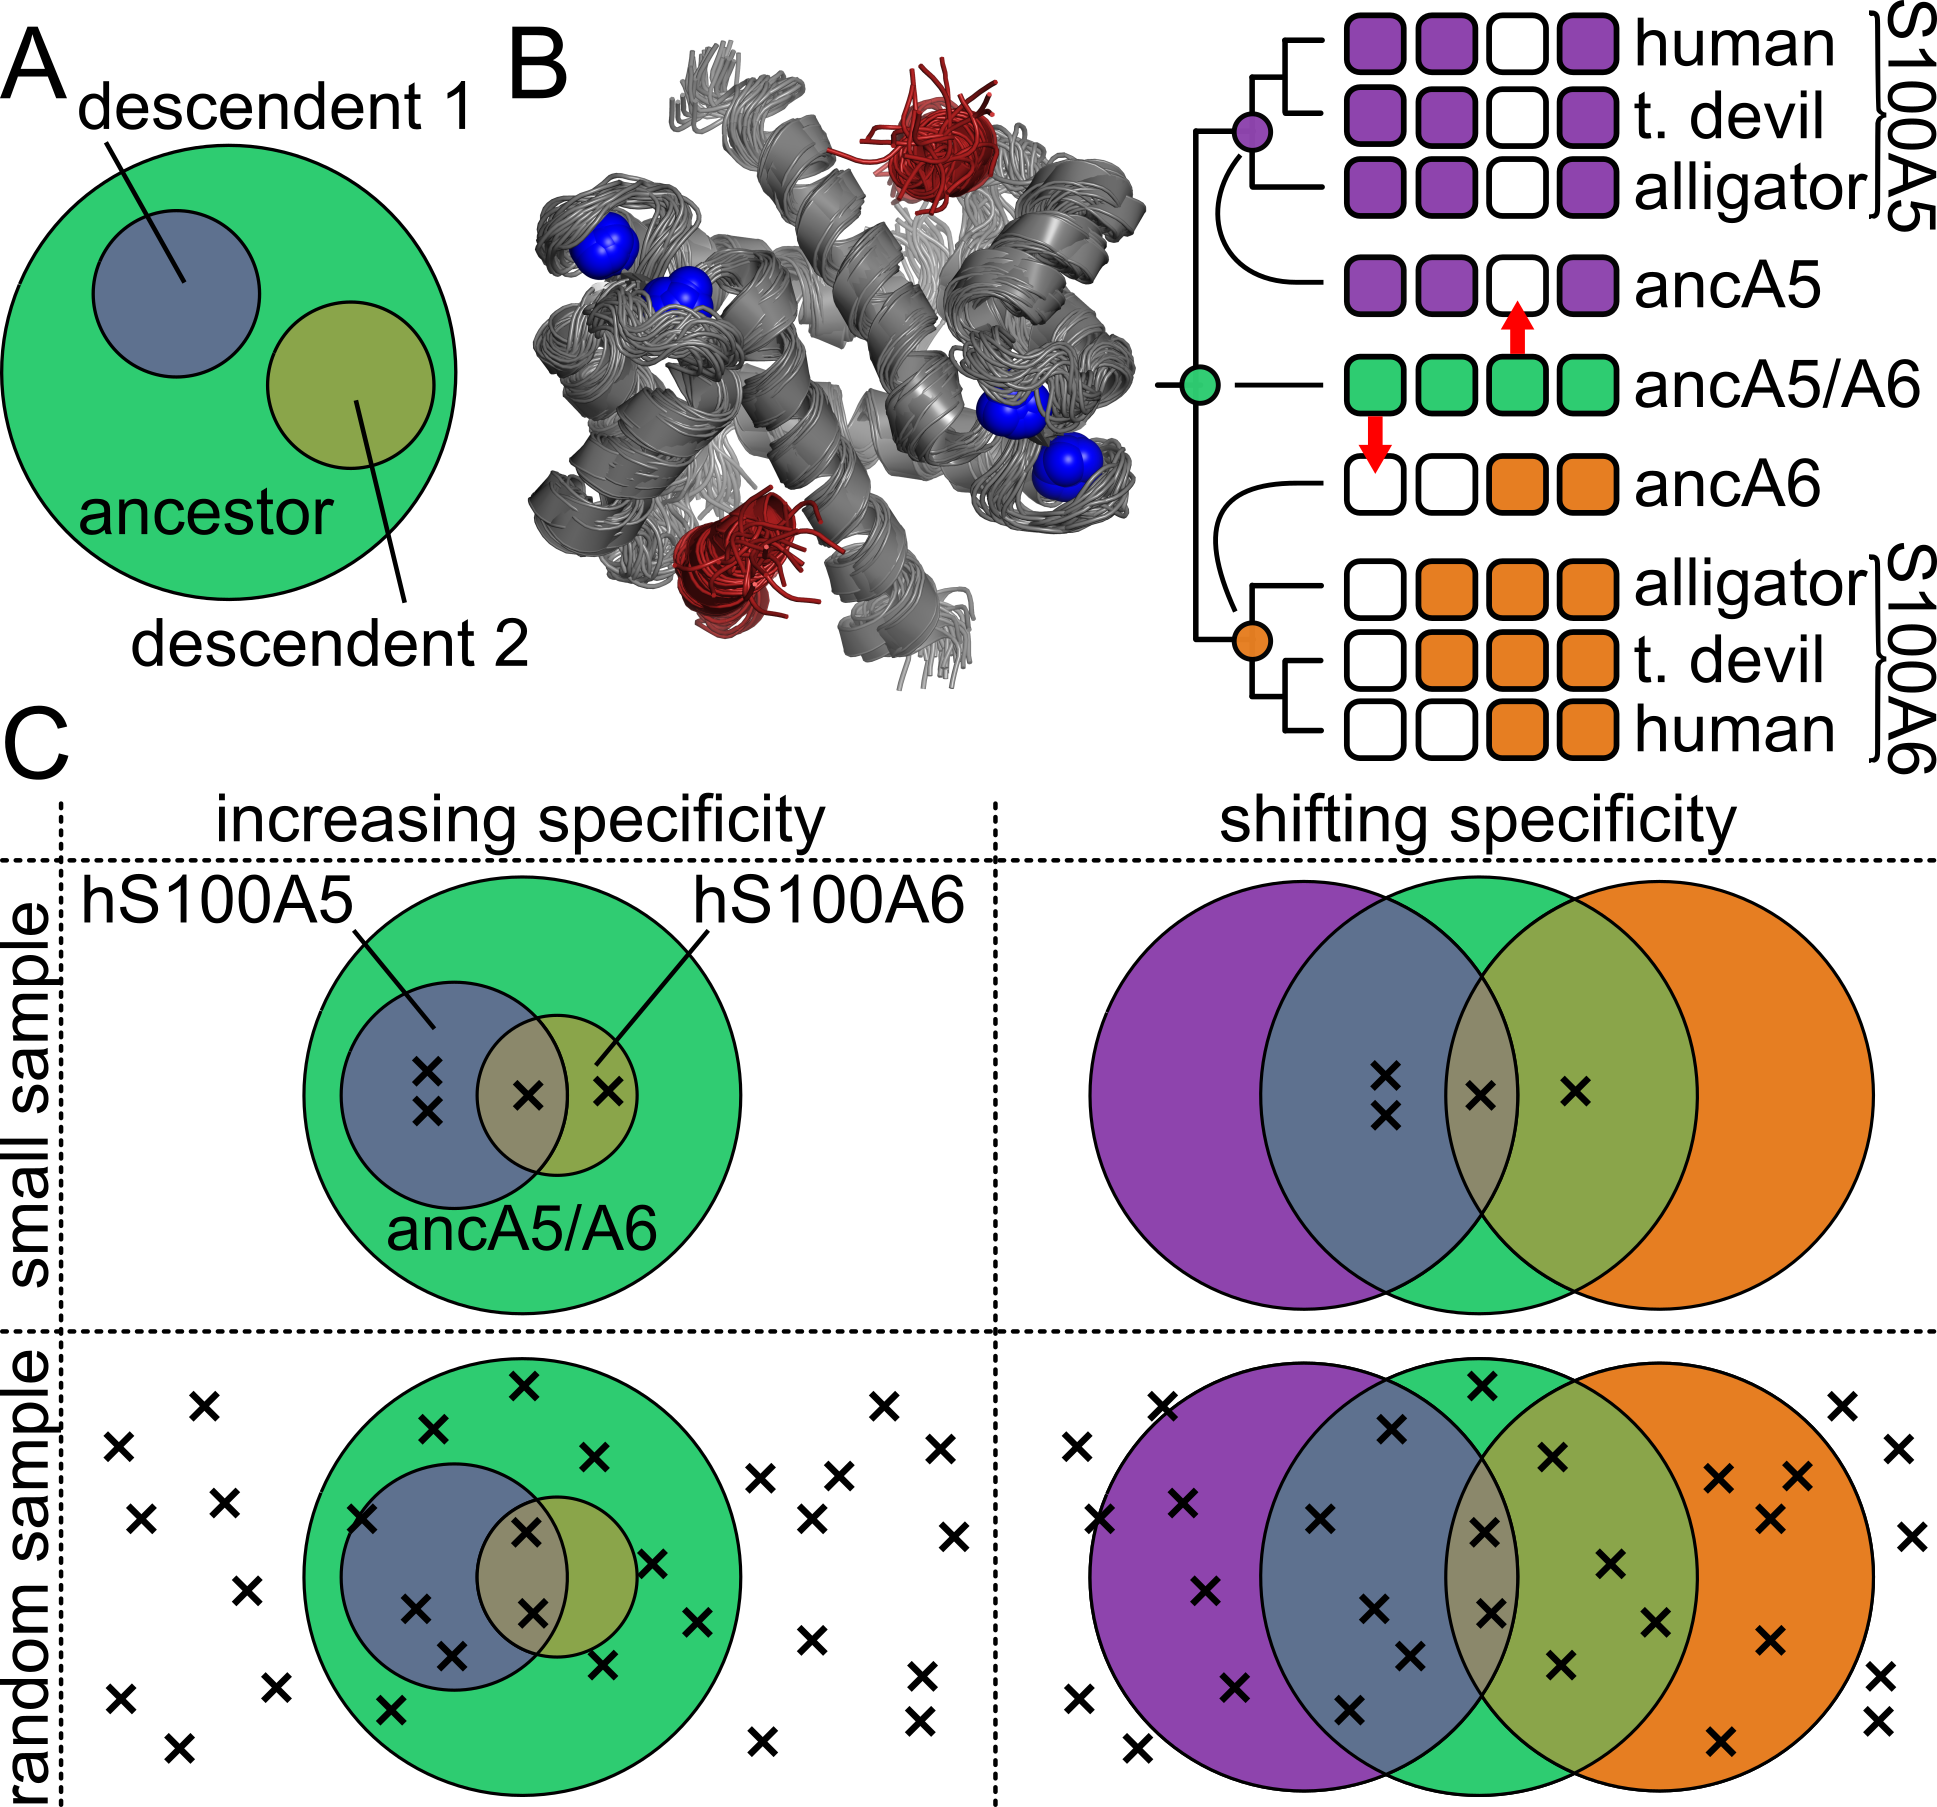
\includegraphics{ch6-fig1.png} 
\caption[Testing the increased specificity hypothesis requires
extensive\newline sampling of targets]{Testing the increased specificity hypothesis requires
extensive sampling of targets. A) Venn diagram of the increasing-specificity
hypothesis. The large circle is set of targets recognized by the ancestor;
the smaller circles are sets of targets represented its descendants.
There is no strict requirement that descendants be subsets of the
ancestor. B) Experimentally measured changes in peptide binding specificity
for S100A5 and S100A6 (taken from \citep{wheeler_conservation_2017}).
Structure: location of peptide (red) binding to a model of S100A5
(gray, PDB: 2KAY). Bound $Ca^{2+}$ are shown as blue spheres. Phylogeny:
Boxes represent binding of four different peptides (arranged left
to right) to nine different proteins (arranged top to bottom). A white
box indicates the peptide does not bind that protein; a colored box
indicates the peptide binds. Colors denote ancA5/A6 (green), S100A5
(purple), and S100A6 (orange). Red arrows highlight ancestral peptides
lost in the modern proteins. C) Venn diagrams show overlap in peptide
binding sets between ancA5/A6, S100A5, and S100A6. Crosses denote
experimental observations. Columns show two evolutionary scenarios:
increasing specificity (left) versus shifting specificity (right).
Rows show to different sampling methods: small sample (top) versus
random sampling (bottom). Colors are as in panel B. \label{samplefigure}}	
\end{figure}

\subsection{Estimating peptide interactions by phage display}

We first assayed the binding of tens of thousands of peptides to each
protein using phage display. We panned a commercial library of randomized
12-mer peptides expressed as fusions with the M13 phage coat protein.
The S100 peptide-binding interface is only exposed upon $Ca^{2+}$-binding
(Fig 19B); therefore, we performed phage panning experiments in the
presence of $Ca^{2+}$ and then eluted the bound phage using EDTA
(Fig 20A). The population of enriched phage will be a mixture of phage
that bind at the site of interest and phage that bind adventitiously
(blue and purple phage, Fig 20A). Peptides in this latter category
enrich in $Ca^{2+}$-dependent manner through avidity or binding at
an alternate site \citep{sidhu_phage_2000,willats_phage_2002}. To
separate these populations, we repeated the panning experiment in
the presence of a saturating concentration of a competitor peptide
known to bind at the site of interest (Fig 20B) \citep{wheeler_conservation_2017}.
This should lower enrichment of peptides that bind at the site of
interest, while allowing any adventitious interactions to remain.
By comparing the competitor and non-competitor pools, we can distinguish
between actual and adventitious binders. 

\begin{figure}%figure 2
\centering
	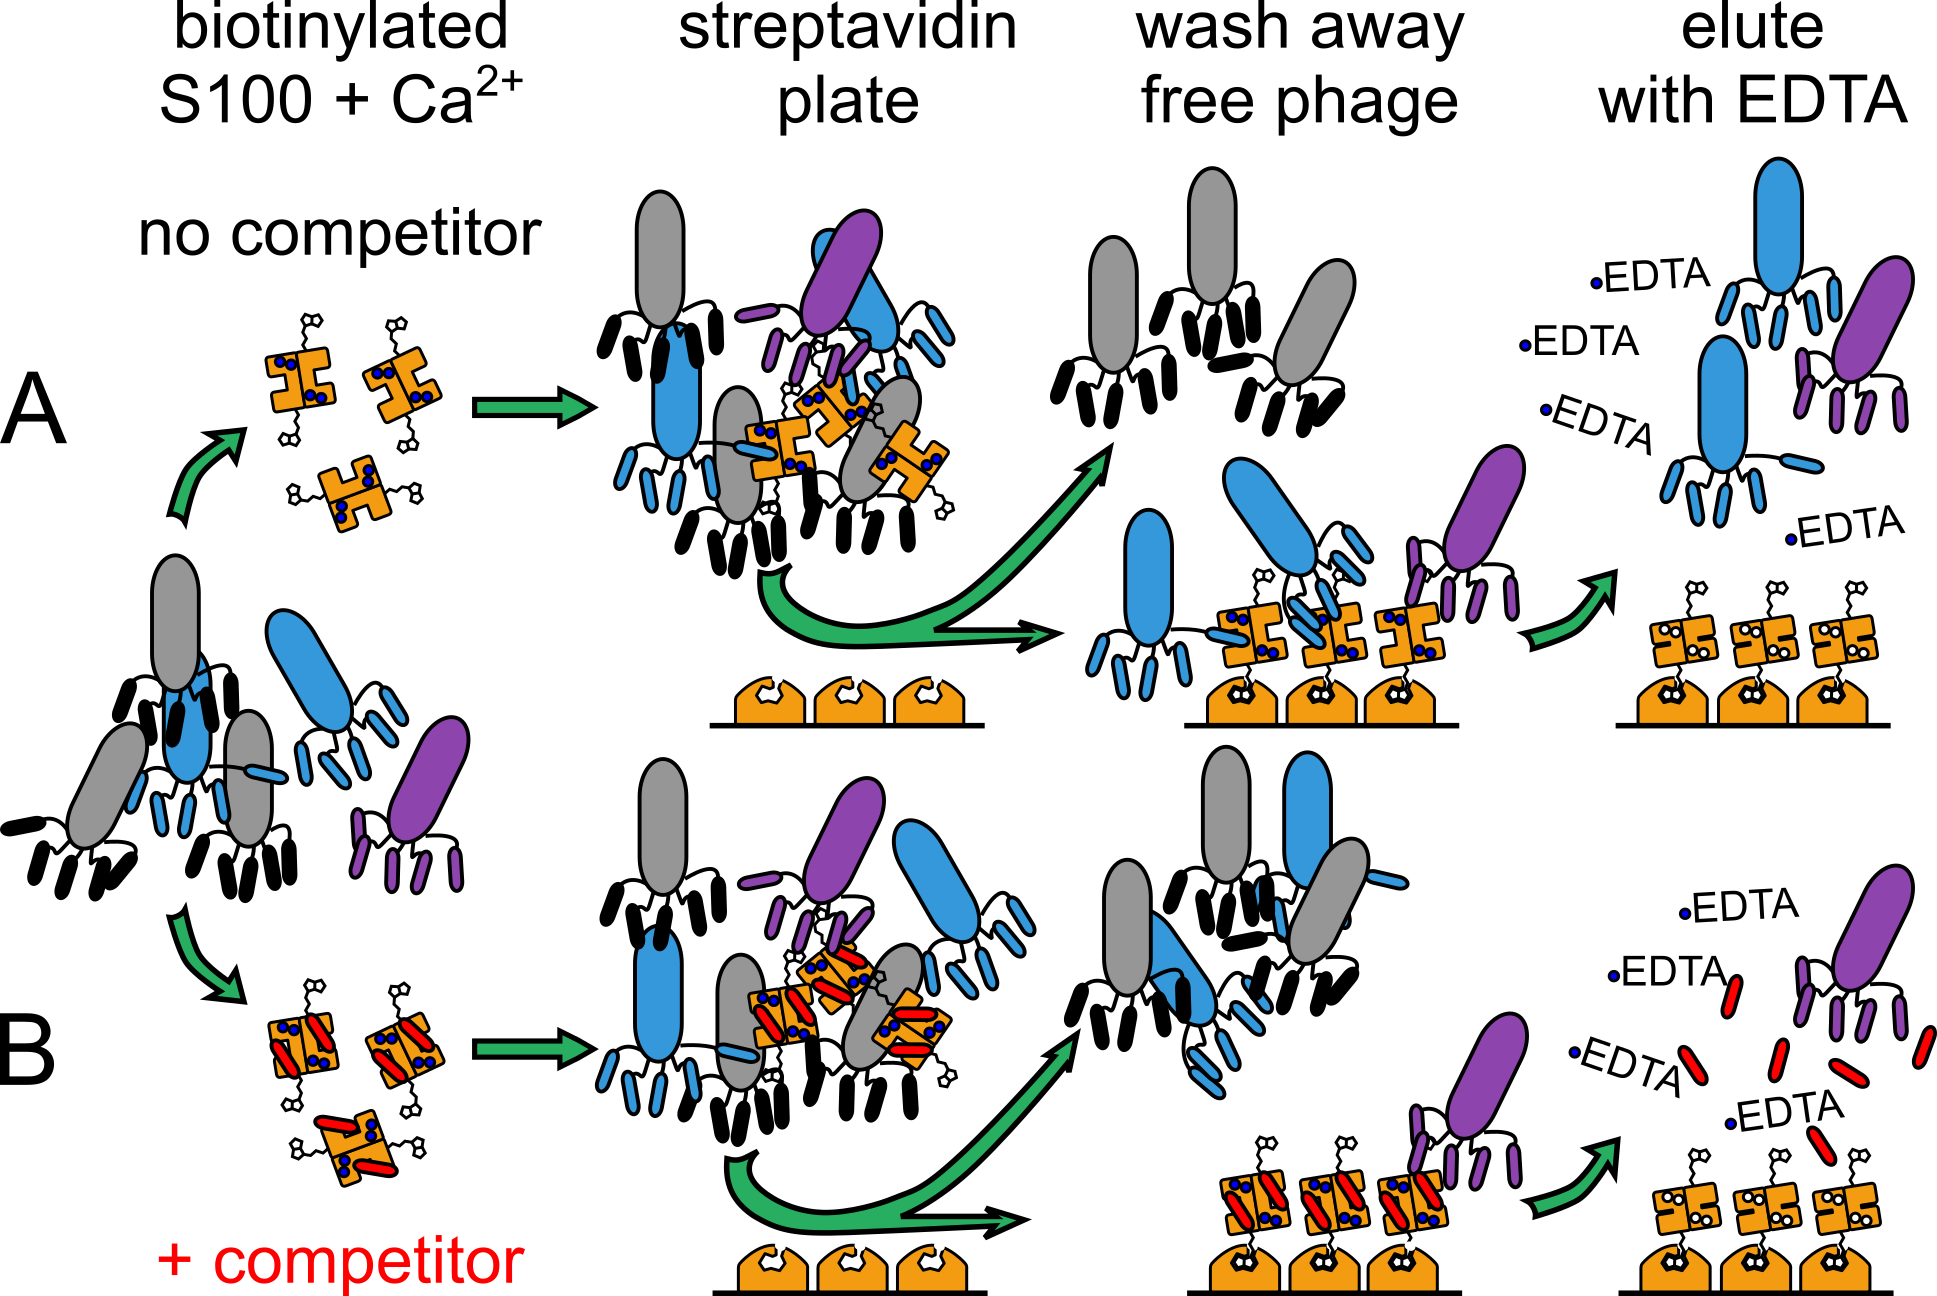
\includegraphics{ch6-fig2.png} 
\caption[Set of binding peptides can be estimated using phage
display.]{Set of binding peptides can be estimated using phage
display. Rows show two different experiments, done in parallel, for
each protein. Biotinylated, $Ca^{2+}$-loaded, S100 is added to a
population of phage either alone (row A) or with saturating competitor
peptide added in trans (row B). Phage that bind to the protein (blue
or purple) are pulled down using a streptavidin plate. Bound phage
are then eluted using EDTA, which disrupts the peptide binding interface.
In the absence of competitor (row A), phage bind adventitiously (purple)
as well as at the interface of interest (blue). In the presence of
competitor (row B), only adventitious binders are present. \label{samplefigure}}	
\end{figure}

We performed this experiment with and without competitor, in biological
duplicate, for hA5, hA6, ancA5/A6, and altAll. We found that phage
enriched strongly for all proteins relative to a biotin-only control
(Fig 35 in supplement). Further, the addition of competitor binding knocked down
enrichment in all samples (Fig 35 in supplement). After panning, we sequenced the
resulting phage pools, as well as the input library, by Illumina.
We applied strict quality control (see methods), discarding any peptide
that exhibited less than six counts (Fig 36 in supplement). After
quality control, we had a total of 265 million reads spread over 17
samples (Table 10 in supplement). 

We estimated changes in the frequencies of peptides between samples
with and without competitor peptide. For each peptide $i$, we determined
$E_{i}=-ln(\beta_{i}/\alpha_{i})$, where $\beta_{i}$ and $\alpha_{i}$
are the frequencies of the peptide in the non-competitor and competitor
samples, respectively. Defined this way, a more negative value of
$E$ corresponds to a larger decrease in peptide frequency upon addition
of competitor peptide. We used a clustering approach to estimate $E$
for $\text{\ensuremath{\approx}}40,000$ different peptides for each
protein. We found that $E$ exhibited a bimodal distribution for all
four proteins, apparently reflecting two underlying processes (Fig
21A, Fig 37 in supplement). The dominant peak consists of ``unresponsive'' peptides
whose frequencies change little in response to competitor peptide.
A second, broader, distribution describes ``responsive'' peptides
whose frequencies change dramatically with the addition of competitor.
There was no systematic difference between estimates of $E$ between
biological replicates (Fig 21B, Fig 38 in supplement). For hA5, the regression line
between replicates has a slope $1.06$ and an intercept of $-0.05$.
This axis of variation explains $\text{\ensuremath{\approx}}81\%$
of the total variation in the data. There are two distinct regions
in the correlation plot, corresponding to the unresponsive and responsive
peptide distributions. The unresponsive distribution forms a large
cloud about zero. In contrast, the responsive peptide distribution
extends along the 1:1 line in a correlated fashion. 

\begin{figure}%figure 3
\centering
	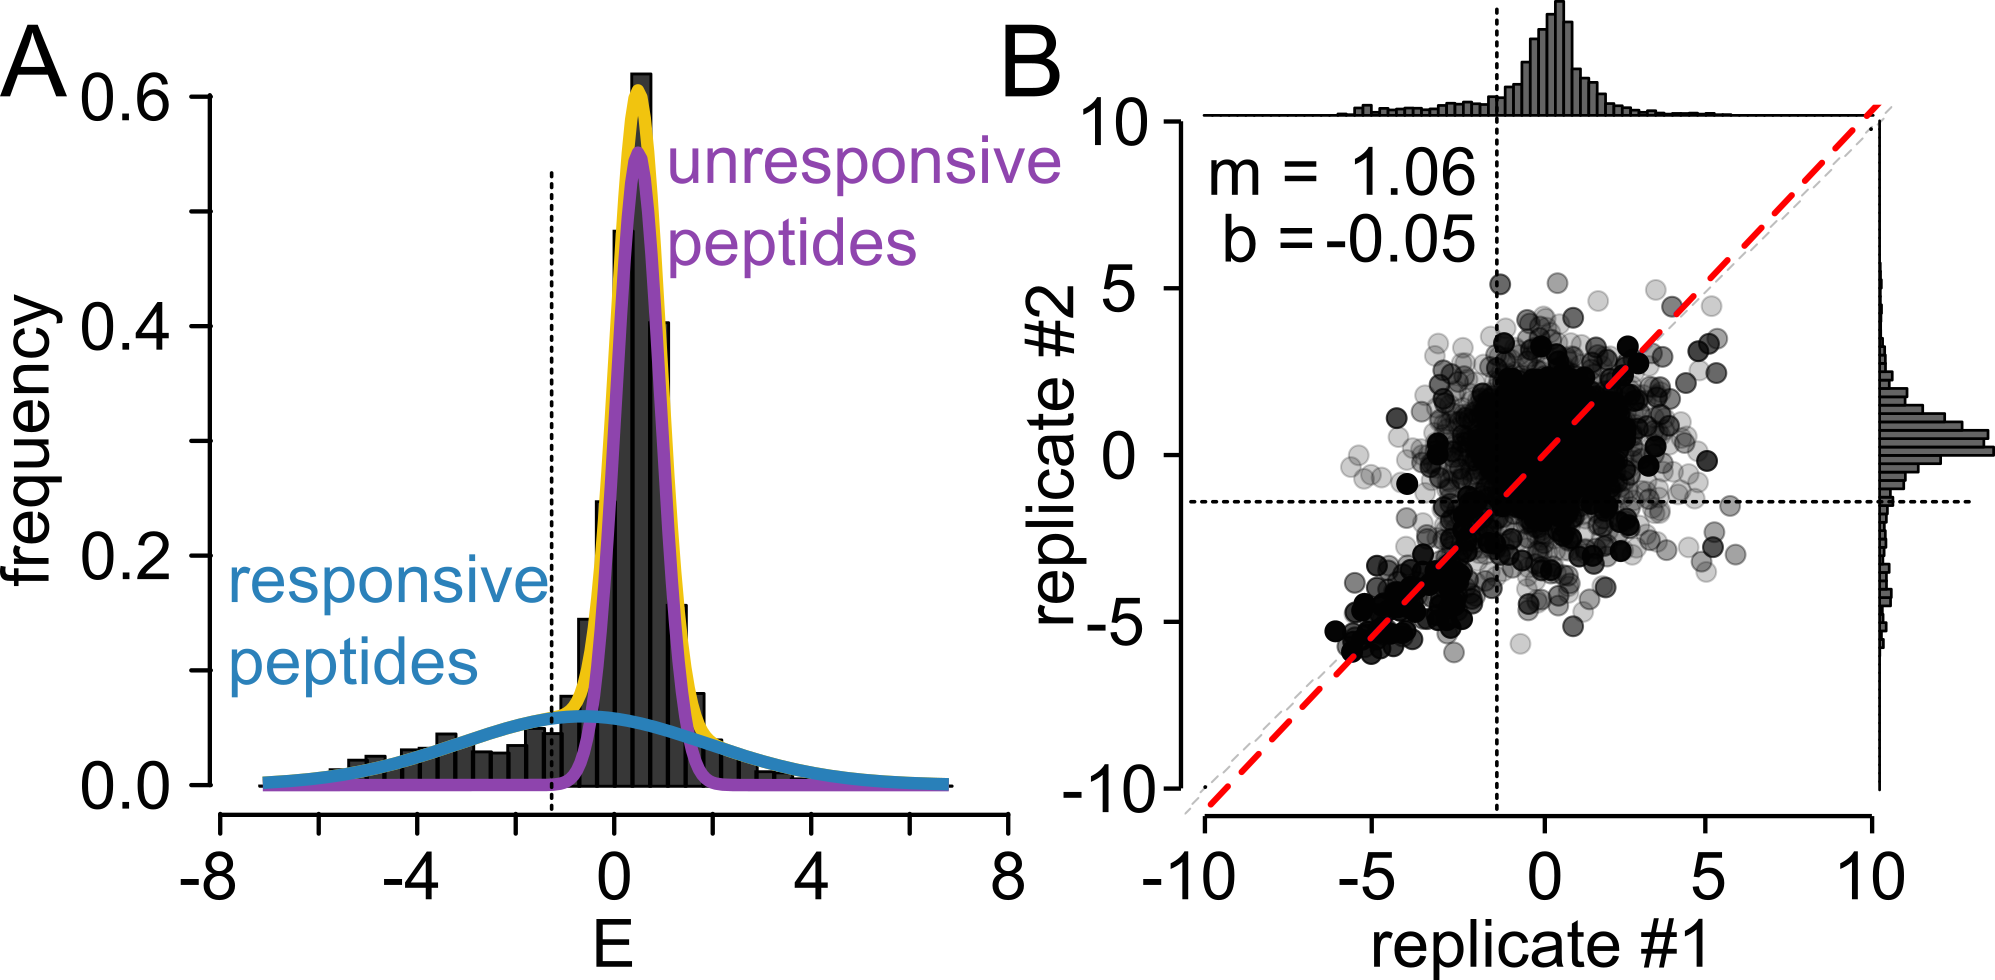
\includegraphics{ch6-fig3.png} 
\caption[A subpopulation of phage respond to addition
of competitor]{A subpopulation of the phage respond to the addition
of competitor peptide. A) Distribution of enrichment values for peptides
taken from pooled biological replicates of hA5. The measured distribution
(gray) can be fit by the sum of two Gaussian distributions: responsive
(blue) and unresponsive (purple), which sum to the total (yellow).
B) Enrichment values from biological replicates are strongly correlated.
Axes are enrichment for replicate \#1 or replicate \#2. Points are
individual peptides. Distributions for each replicate are shown on
the top and right, respectively. The red dashed line is the best fit
line (orthoganol distance regression), explaining $\approx$81\% of the
variation in the data.\label{samplefigure}}	
\end{figure}

\subsection{Supervised machine learning allows prediction of binding}

Our phage display experiment yielded a collection of peptides whose
enrichment is disrupted by competitor, however, this information is
not sufficient to construct the desired Venn diagram. First, a Venn
diagram requires knowing the binding for a common set of peptides
to all proteins. Because the total sets of partners are large for
all proteins, we observed different peptides in each experiment (hA5
vs. hA6 vs. ancA5/A6 vs. altAll). Second, phage display is an imperfect
proxy for binding. It has confounding non-biological factors: peptides
are in the context of phage particles, the protein becomes immobilized
by a biotin tag, there is the possibility of avidity, and enrichment
is determined by off-rate rather than equilibrium. 

To solve these issues, we sought to relate our measured $E$ for these
peptides back to binding of a common set of peptides. We used supervised
machine learning to train models to predict binding from amino acid
sequence for each protein. We then applied each model to an identical
set of peptides, allowing us to directly compute a Venn diagram for
peptide specificity. 

We trained our models against 57 chemical features that we could could
readily calculate from an amino acid sequence. These included measures
of hydrophobicity, hydrogen bonding, geometry, secondary structure
propensity, and electrostatics. In addition to these specific features,
we also defined 20 ``meta'' features by taking the principle components
of the entire aaindex database \citep{kawashima_aaindex:_2008}, which
reports 590 quantitative values for each of the 20 amino acids. For
most chemical features, we simply added the values for each amino
acid in a sequence. For example, we would sum up the number of hydrogen
bond donors across the sequence and treat that as a chemical feature.
We also used CIDER to calculate a few non-additive electrostatic features
for each sequence \citep{holehouse_cider:_2015}, such as the isoelectric
point. A full list of the features we calculated is given in Table 11 (in supplement). 

We calculated these 57 features for the entire sequence and for all
sliding windows ranging from 1 to 11 amino acids (Fig 22A). This introduces
neighbor-neighbor correlation between features that improves model
power. Overall, we calculated the features for 78 sliding windows
on each peptide, giving us a total of $57\times78=4,446$ features
per sequence (Fig 22A). We then trained a random forest regression
model to predict $E$ using the features of the $\text{\ensuremath{\approx}}40,000$
we observed for each protein. A random forest model finds weights
for a collection of random decision trees based on a set of input
features \citep{breiman_random_2001}. Prior to training, we withheld
10\% of the peptides as a test set. We then optimized nuisance parameters
such as the number of trees and choice of data weighting scheme using
k-fold cross validation within the training set ($k=10$). After training,
the $R^{2}$ between our model and the training set was $\approx97\%$
for all proteins (Table 2). 

\begin{table}[h!]\footnotesize
\center
\scriptsize
\caption[Protein binding model statistics] {Protein binding model statistics.}
\scriptsize
\begin{tabular}{c|c|ccc|cc}
protein & num. training observations & $R_{train}^{2}$ & $R_{test}^{2}$ & AUC & FPR & FNR\tabularnewline
\hline 
hA5 & 40,887 & 97.6 & 85.1 & 98.9 & 0.35 & 0.35\tabularnewline
hA6 & 42,156 & 97.4 & 82.9 & 96.1 & 0.41 & 0.41\tabularnewline
ancA5/A6 & 43,938 & 97.7 & 84.2 & 97.4 & 0.35 & 0.35\tabularnewline
altAll & 51,903 & 96.6 & 80.0 & 95.1 & 0.45 & 0.15\tabularnewline
\end{tabular}
\end{table}

After our final optimization, we tested our models against their test
sets. $R^{2}$ for test sets ranged from $80-87\%$ (Fig 22B, Table
1). For all models, the regression line reveals a slope slightly greater
than one (e.g. 1.16 for hA5, Fig 22B). Further, the scatter is nonrandom,
with the most negative values of $E$ being overestimated and the
most positive values underestimated. This makes intuitive sense, as
the best-of-the-best and the worst-of-the-worst enriching sequences
likely depend strongly on details not captured by our rather crude
amino acid model. 

\begin{figure}%figure 4
\centering
	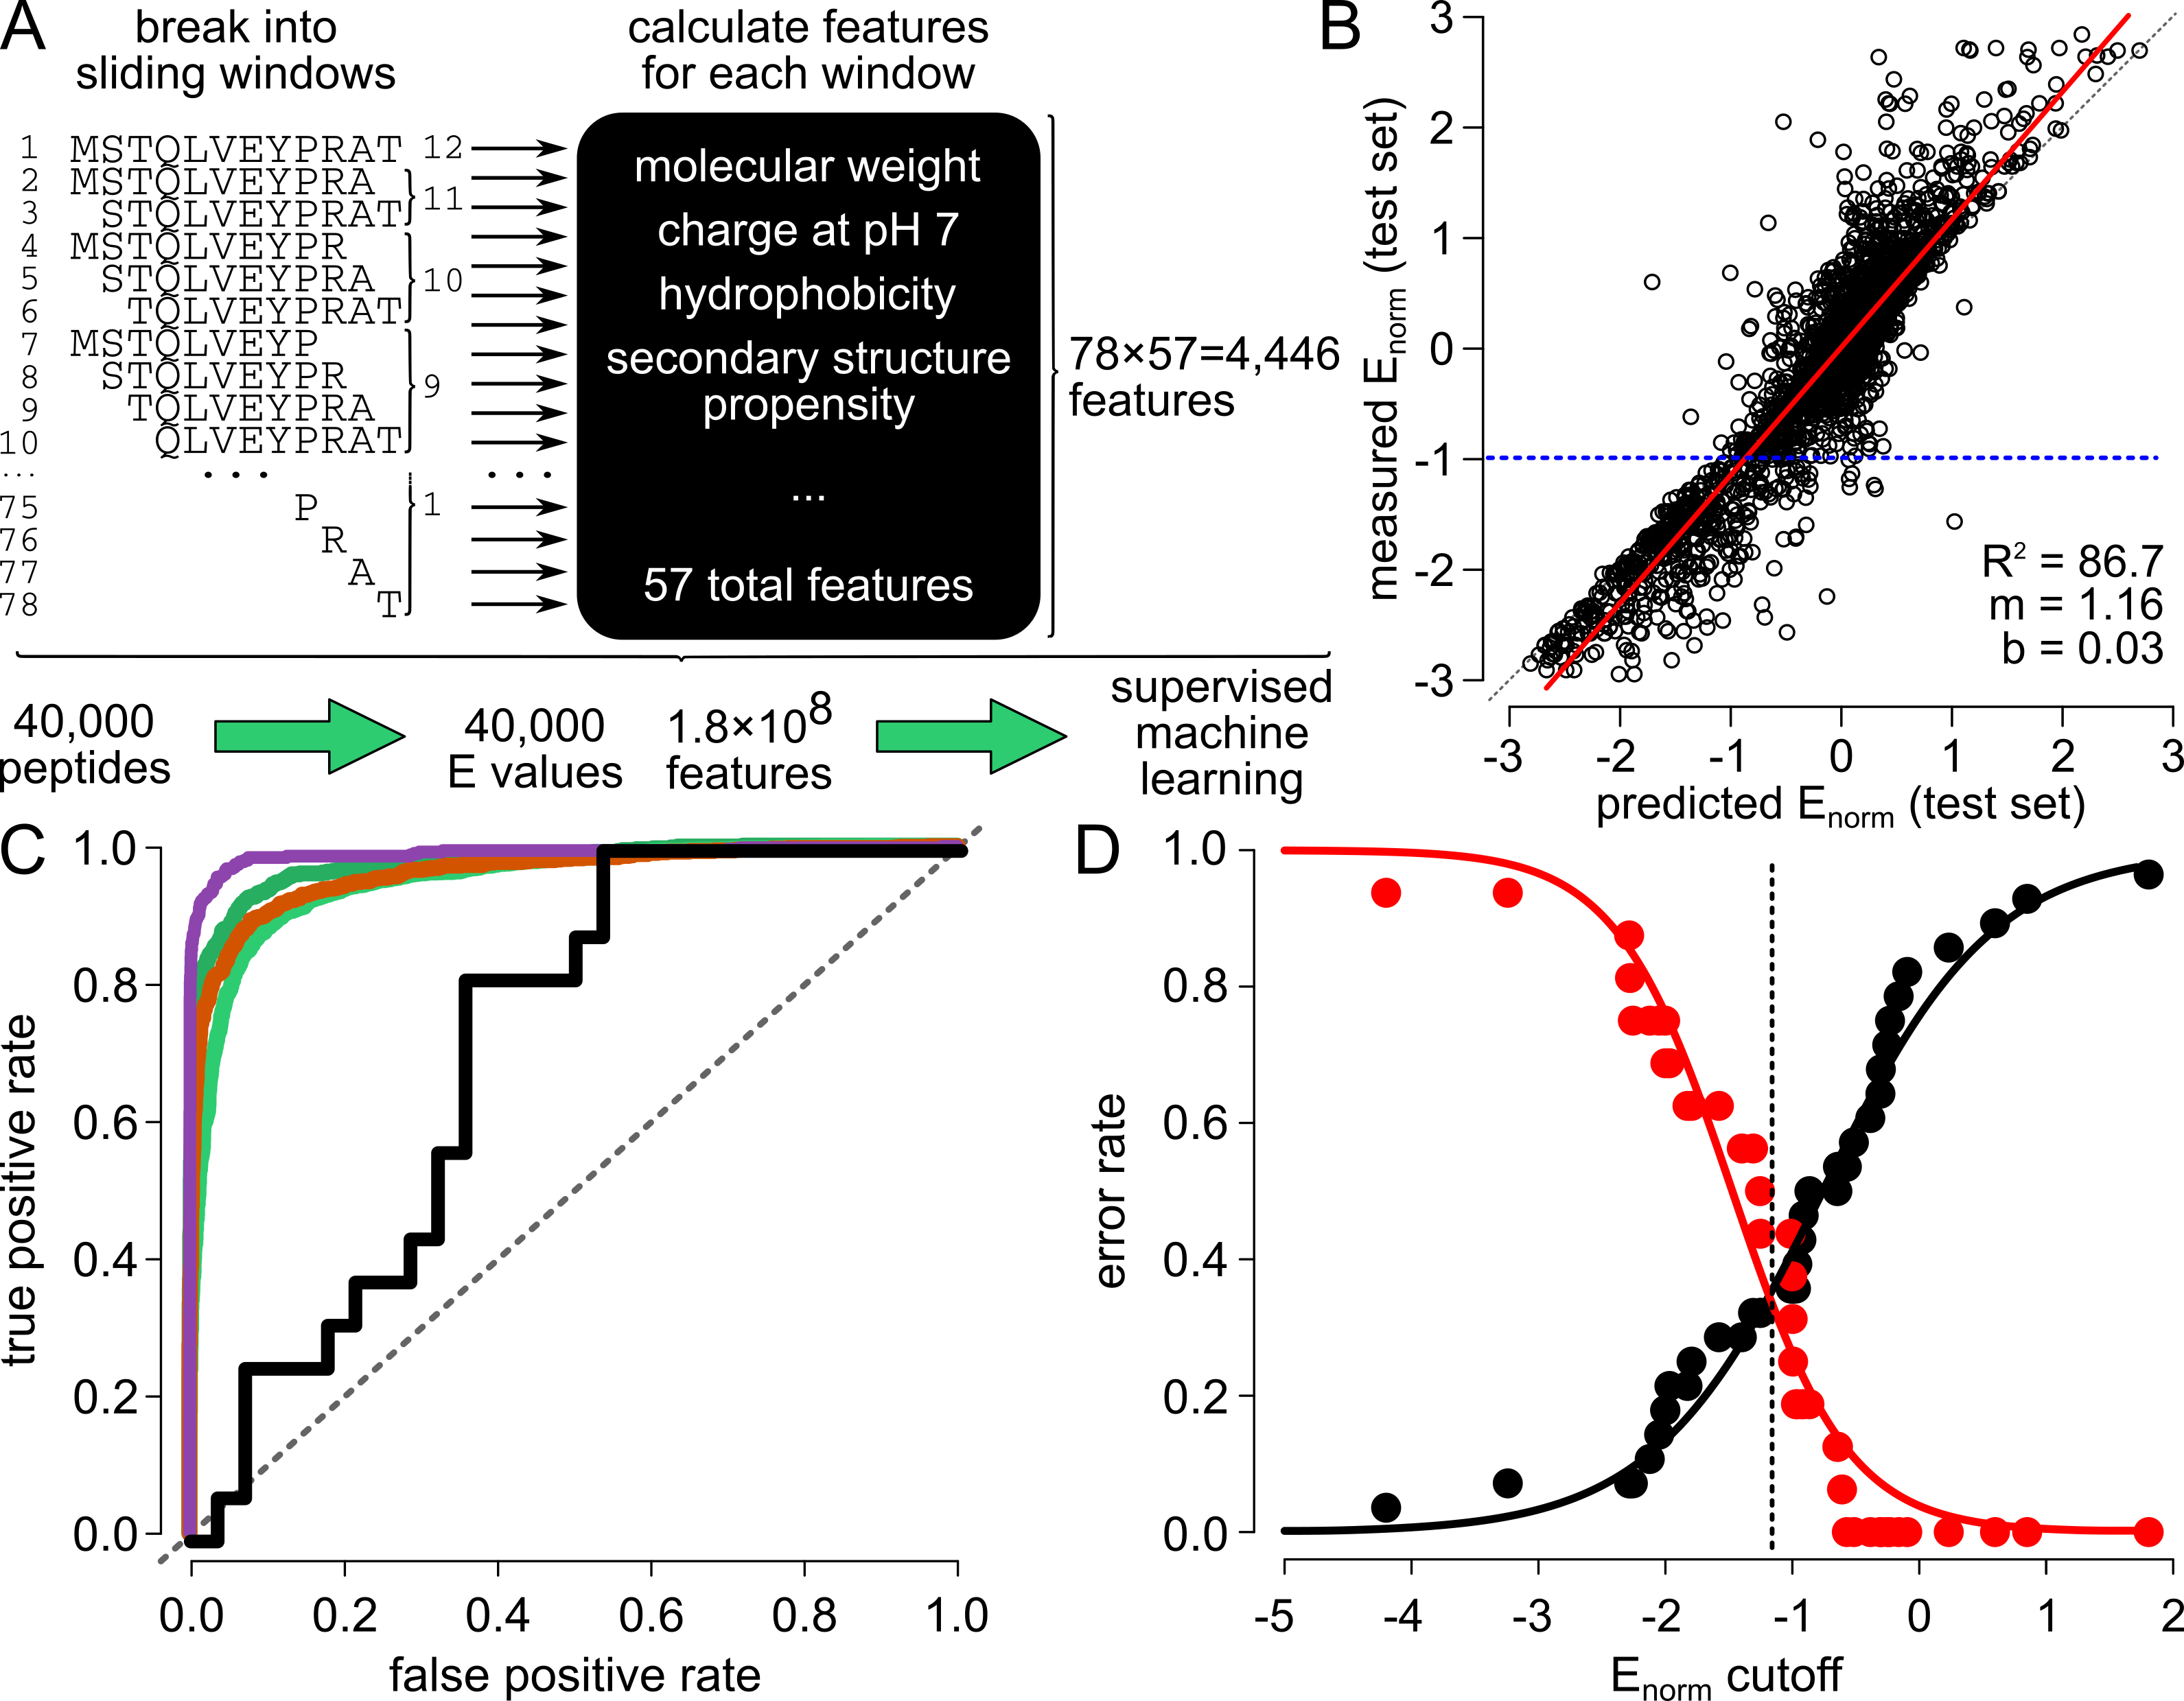
\includegraphics{ch6-fig4.png} 
\caption[Peptide binding can be predicted from amino acid sequence]{Peptide binding can be predicted from amino acid sequence. A) Schematic showing our strategy for training a binding model. We
break the 12-mer peptide into 78 different sliding windows. For each
peptide, we calculate 57 features (black box), giving a total of 4,446
features per peptide. We then use 40,000 peptides to train a model
predicting $E$ (green arrows). B) Correlation between predicted $E_{norm}$
and measured $E_{norm}$ for $\approx$4,000 peptides in test set for
hA5. Each point is a peptide. Red line is least squares regression
line. Blue dashed line is our classification line (see panel C). C)
Receiver Operator Characteristic (ROC) curves for binding models.
Colored series show ability of models to classify measured $E_{norm}$
as $\le$ $-1$ (the blue dashed line form panel B). Curves are hA5 (purple),
hA6 (orange), ancA5/A6 (dark green), and altAll (light green). Black
line is the ROC curve for predicting the binding of 44 isolated peptides.
D) Error rates for predicting isolated peptides that bind as function
of $E_{norm}$ cutoff for the classifier. False negative rate (red)
and false positive rate (red) cross at $E_{norm}$ = $-1.19$ (dashed line)
with a value of $\approx$0.35. Solid lines are fits of the modified
Hill equation to the to error rates.\label{samplefigure}}	
\end{figure}

To calculate a Venn diagram, we need to classify peptides as binders
or non-binders. We therefore tested how well our models would operate
as classifiers. To facilitate this comparison, we normalized $E$
for each protein such that the competitor peptide had an enrichment
value of -1. We did this by $E_{norm}=E/|E_{comp}|$, where $E_{comp}$
is the enrichment of the competitor peptide. We then asked whether
our models could predict if peptides in the test set had measured
$E_{norm}<-1$. We then attempted to classify peptides into the categories
$E_{norm}<-1$ vs. $E_{norm}\ge-1$. 

We swept along cutoffs in predicted values of $E_{norm}$ and calculated
our false positive and false negative rate using the measured values
of $E_{norm}$ for test-set peptides. As expected, increasing the
cutoff increased the false positive rate and decreased the false negative
rate for each model. We quantified this behavior with Receiver Operator
Characteristic (ROC) curves. A ROC curve is a plot of the true positive
rate against the false positive rate as one changes the classifier
cutoff. A perfect predictor will have a cutoff value where the false
positive rate is 0 and the true positive rate is 1. As a consequence,
the Area Under the Curve (AUC) will be 1.0. In contrast, a random
predictor will follow the 1:1 line and will have an AUC of 0.5. All
of our models had steep ROC curves that gave AUC values from 0.95
to 0.99 (Fig 22C). Given the amino acid sequence of a 12-mer peptide,
we can therefore predict with high confidence whether a peptide will
respond to the addition of competitor peptide in a phage display experiment. 

We next set out to calibrate our phage enrichment values against binding
of isolated peptides. We did this by calculating $E_{norm}$ for 44
peptide/protein pairs and then measuring their binding using Isothermal
Titration Calorimetry (Table 12 in supplement). We used 17 peptides, some with known
binding properties \citep{lee_structure_2008,streicher_annexin_2009,liriano_structure_2012},
others that were in the freezer for other projects, and still others
were extracted from the human proteome as possible S100 targets. We
measured binding of 16 of these peptides to hA5, 13 to hA6, 8 to ancA5/A6,
and 6 to altAll. We classified any peptide with a measurable binding
constant ($K_{D}$ $\apprle$100 $\mu M$) as ``binding'' and all others
as ``non-binding.'' 

We then swept along $E_{norm}$ and attempted to classify the 44 measured
binders. The ROC curve came off the diagonal, with an AUC of 0.71
(Fig 22C). While this is significantly worse than the predictions of
$E_{norm}<-1$, it is not unexpected given that we trained our model
on phage display data and are now attempting to use it to predict
isolated peptide binding. To verify that this low AUC curve indicated
real binding signal, we simulated 44-observation ROC curves using
a random predictor. We found that the probability of observing an
AUC of 0.71 or greater by chance was 0.007---a strong indication that
there is signal in our binding model. 

To identify a cutoff for predicting binders, we plotted the false
positive rate and false negative rate against $E_{norm}$ for all
44 peptides. We then identified the value of $E_{norm}$ that simultaneously
minimized the false positive and false negative rates. To estimate
the crossover point, we fit the modified Hill equation to each curve,
which empirically captures the basic shape of these curves. We found
that these curves crossed for $E_{norm}=-1.19$, with false positive
and false negative rates of $\approx$0.35. These rates are high and
therefore preclude confidently predicting whether a specific peptide
binds. This is, however, sufficient to determine a Venn diagram for
the binding specificity of these proteins. 

\subsection{Venn diagrams can be estimated using MCMC}

We next used our trained and calibrated models to estimate the Venn
diagram describing the binding sets for the modern and ancestral proteins
(Fig 19). We applied our models for hA5, hA6, ancA5/A6, and altAll
to a common collection of 1,000,000 random 12-mer peptides, classifying
any peptide with $E_{norm}<-1.19$ as binding. We then calculated
the overlap between these sets, placing the counts for each region
of the Venn diagram into the vector $\vec{V}_{obs}$. 

Because we have high (and uncertain) false positive and false negative
rates, the counts in $\vec{V}_{obs}$ may not be identical to the
real populations of the Venn diagram ($\vec{V}$). We therefore sampled
over counts in $\vec{V}$, as well as possible false positive and
false negative rates, using Bayesian Markov Chain Monte Carlo (MCMC).
We wrote a transition matrix ${\bf T}$ that maps $\vec{V}$ into
$\vec{V}_{obs}$ ($\vec{V}_{obs}=\vec{V}\cdot{\bf T}$). ${\bf T}$
defines the probability of each class of miss-call given all false
positive and false negative rates. For example, one element in ${\bf T}$
encodes the probability that we mistakenly identify a hA5-specific
peptide as a hA6-specific peptide (e.g. the false negative rate for
hA5 times the false positive rate for hA6). The details of matrix
construction are given in the supplemental text. 

We allowed each protein to have its own false positive and false negative
error rates. We set the prior probabilities for error rates by estimating
the false positive and false negative rate for binding to each protein
at the cutoff of $E_{norm}<-1.19$ (Fig 39 in supplement). We
then used MCMC to sample values of $\vec{V}$ and the error rates,
comparing the resulting vector to $\vec{V}_{obs}$. We ran two samplers
in parallel until convergence ($\text{\ensuremath{\approx}}2$ million
steps each). This allowed us to estimate both the Venn diagram and
our uncertainty in its composition. 

\subsection{hA5 is more specific than hA6 or the ancestor}

We found that the total size of each binding set ranged from 1.3\%
{[}0.9,1.8{]} of peptides (for hA5) to 22.6\% {[}21.8,22.9{]} of all
peptides (for the altAll construct) (Fig 23). The values in the brackets
denote the 95\% credibility region from the posterior distribution.
The large sizes of these sets likely reflects the low-specificity,
hydrophobic nature of the S100 binding interface \citep{wheeler_conservation_2017}. 

\begin{figure}%figure 5
\centering
	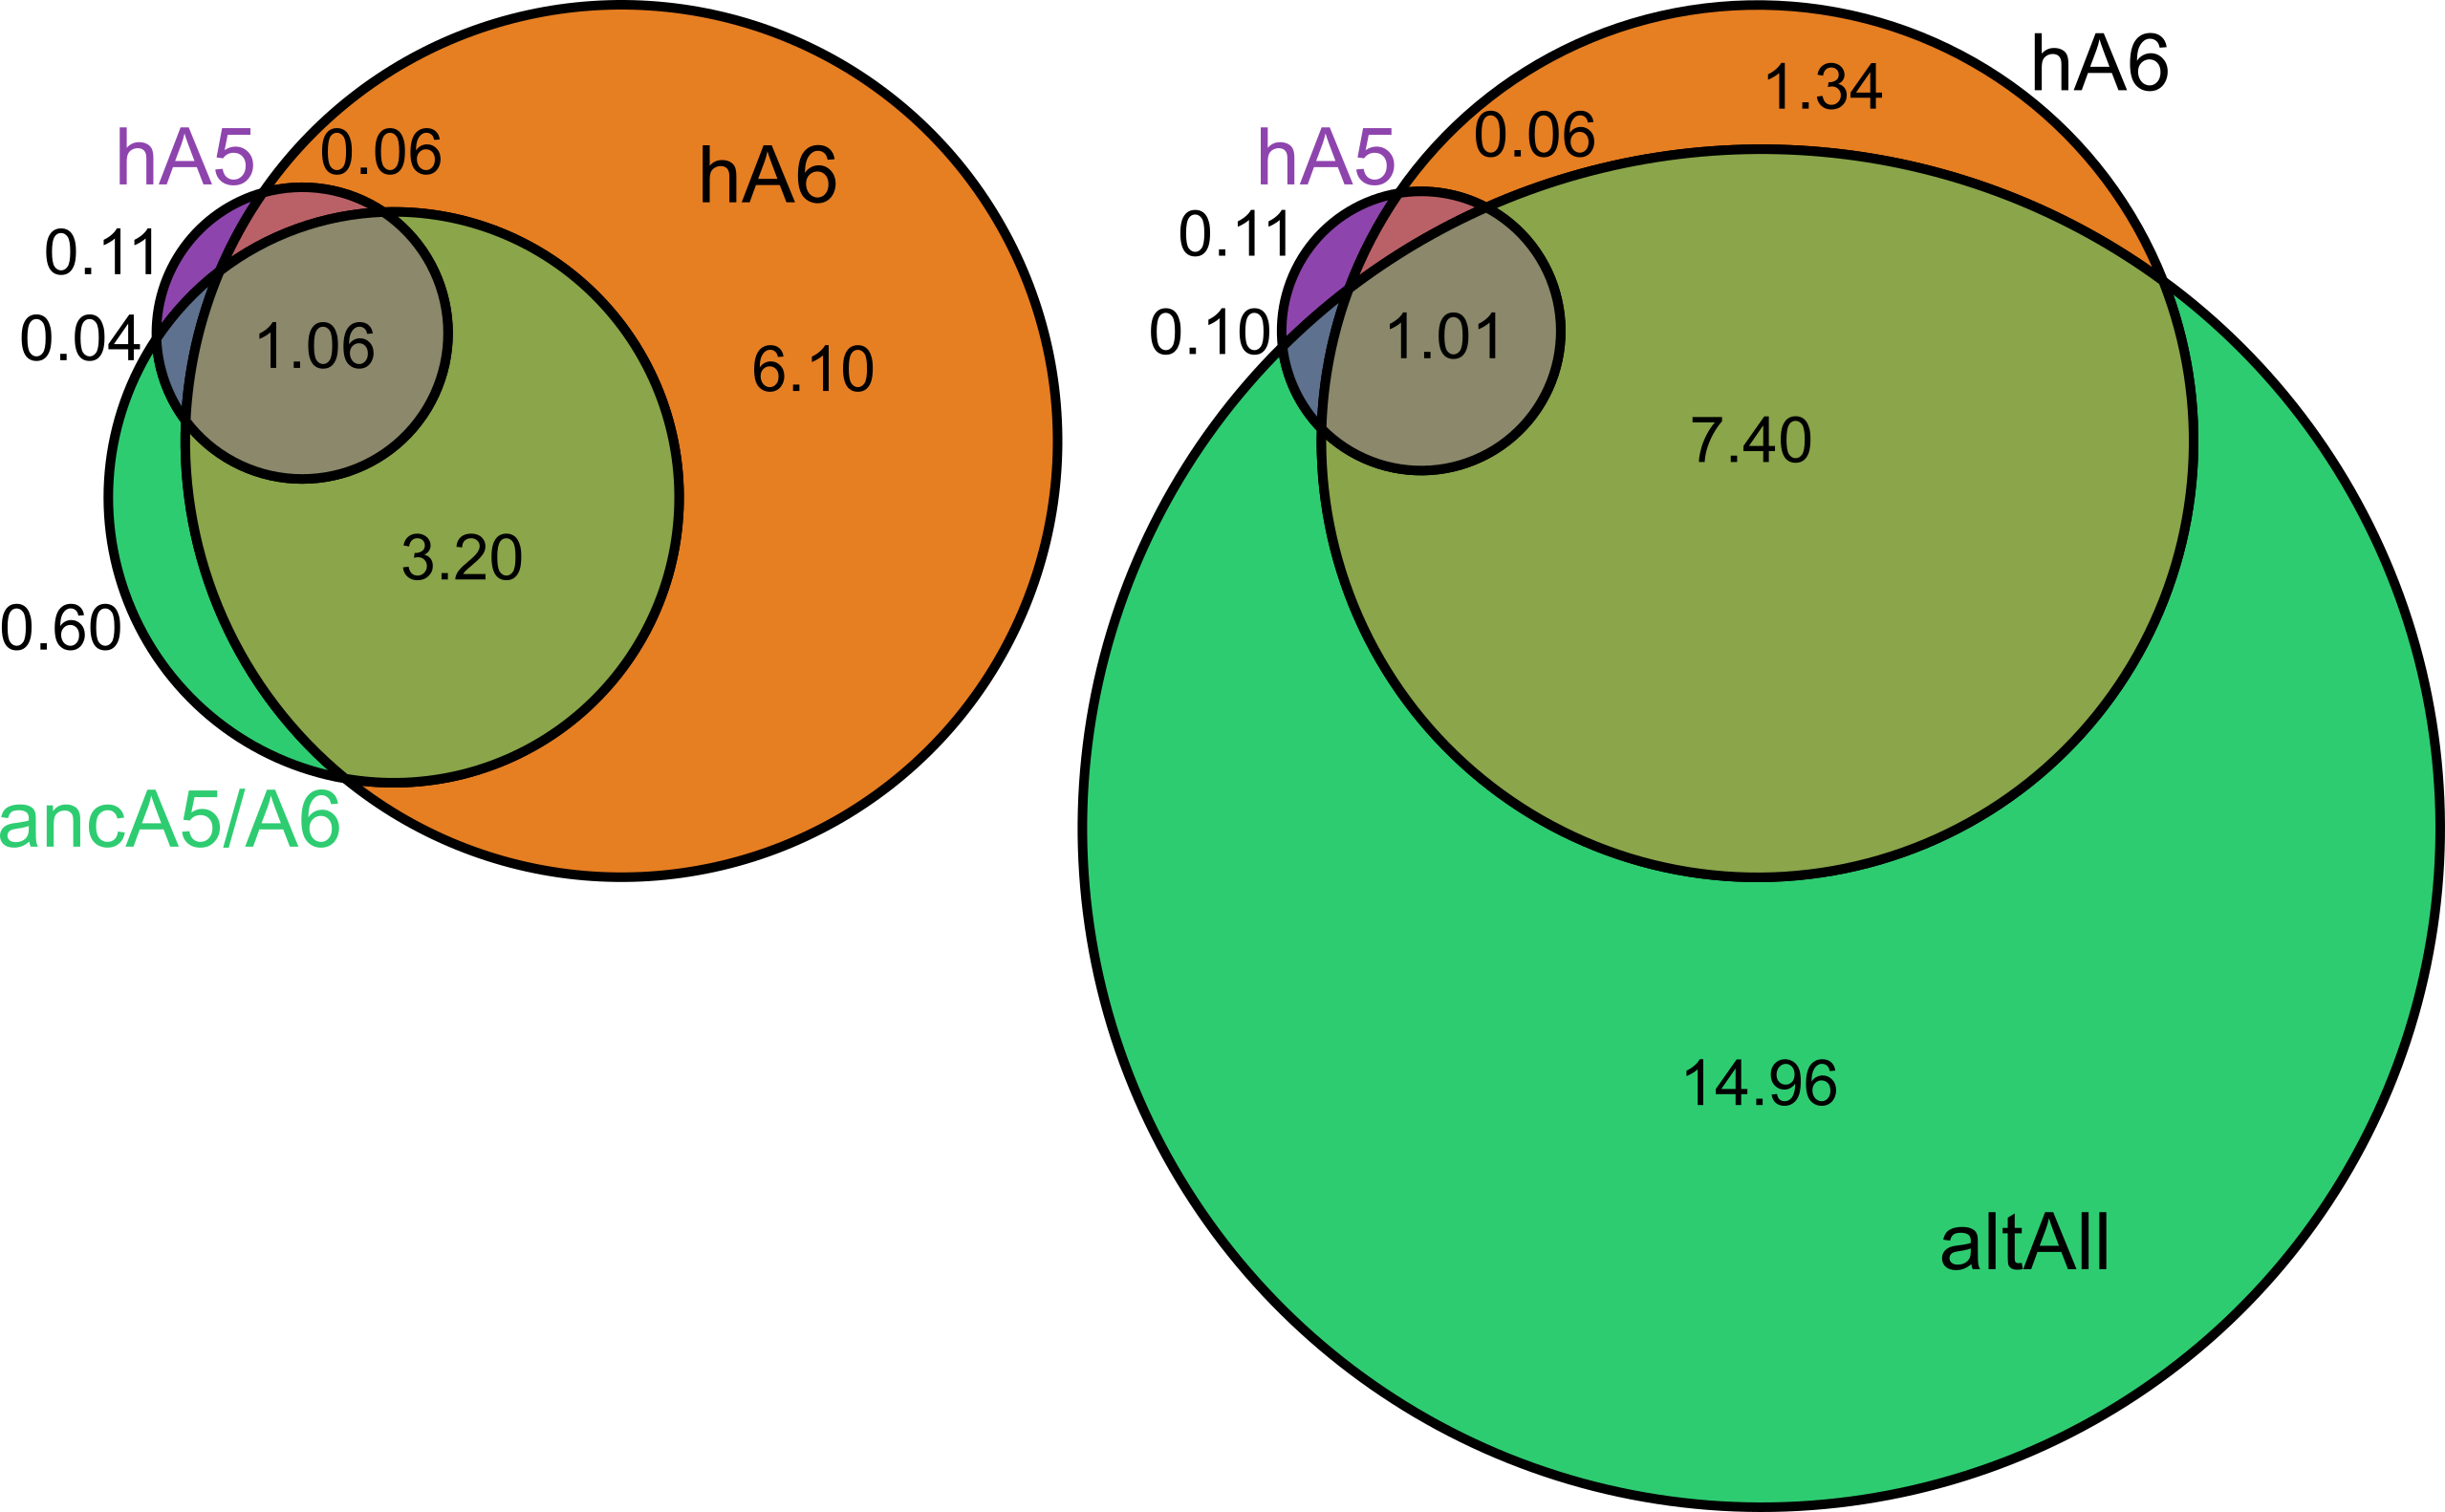
\includegraphics{ch6-fig5.png} 
\caption[Changes in binding sets over time]{Changes in binding sets over time. Circles denote
estimated binding sets for hA5 (purple), hA6 (orange), or ancestors
(green). Areas and numbers in each region indicate the percent of
random peptides in that region of the Venn diagram. The left panel
shows the maximum likelihood ancestor (ancA5/A6); the right panel
shows the altAll reconstruction.\label{samplefigure}}	
\end{figure}

We found that hA5 exhibits increased specificity relative to the ancestral
proteins, apparently evolving by a process of subfunctionalization.
The hA5 peptide set is a subset of the ancestral binding set (Fig
23). While $\text{\ensuremath{\approx}}85\%$ of peptides are shared
with the ancestor, only $\text{\ensuremath{\approx}}9\%$ of peptides
arose specifically for binding to hA5. This result is robust to phylogenetic
uncertainty, as very similar overlaps are observed for ancA5/A6 (86.5\%
{[}83.9,95.2{]}) and the altAll construct (84.6\% {[}81.1,91.4{]}).
The hA5 peptide set was also largely a subset of the hA6 set: 80.6\%
{[}76.8,88.5{]} of hA5 peptides are also hA6 peptides. This demonstrates
that, although the protein has subfunctionalized from the ancestor,
it has constricted onto a set of peptides that mostly overlaps with
the paralogous hA6 (Fig 23). 

The results for hA6 depend on the reconstruction used for the ancestral
state. The hA6 binding set was much larger than hA5---consisting of
10.1\% {[}9.2,11.7{]} of peptides. This is is expanded relative to
the ancA5/A6 set. While there is a extensive overlap (37.4\% {[}36.4,38.4{]}),
most hA6 binding targets were acquired after gene duplication (Fig
23). Fully 62.0\% {[}61.1,63.1{]} of peptides are unique to hA6. In
this scenario, hA6 kept its ancestral partners, and then added a large
collection of new partners. However, this pattern varies when inferred
using the altAll construct. 82.9\% {[}80.6,85.2{]} of hA6 peptides
are shared with the altAll ancestor (Fig 23). Under this alternate
scenario, hA6 binding specificity is the result of both subfunctionalization
and the acquisition of new binding partners distinct from the ancestor
(neofunctionalization). Subfunctionalization in this scenario appears
to have occcurred to a far lesser extent than in the paralogous hA5
lineage, with the hA6 binding set representing only a minor constriction
of the ancestral set. However, the maximum likelihood scenario is
strongly supported over the alternative one. Furthermore, the overall
distribution of enrichment values for the altAll construct was systematically
lower than that for any other protein. This result suggests that the
alternate construction may actually have compromised---rather than simply
distinct---activity. 

The alternate reconstruction is a very agressive attempt to incorporate
phylogenetic uncertainty. In this case, the altAll protein differs
at 21 sites from the maximum-likelihood ancA5/A6 and has a much lower
likelihood. The results for hA5 are not changed between these estimates,
but the interpretation of hA6 does differ. Thus it is difficult to
conclude the exact nature of the transition that occurred along the
hA6 lineage. Nonetheless, it is clear that the patterns observed along
the hA5 and hA6 lineages are distinctly different. The transitions
in specificity that occurred following gene duplication are more nuanced
than a simple partitioning of ancestral binding partners across desecendant
proteins. 

\section{Discussion}
Previously, we used a low-throughput approach to characterize the
evolution of the biochemical specificity of S100A5 and S100A6 \citep{wheeler_conservation_2017}.
We observed a strong signal of phylogenetic conservation in the pattern
of peptide binding specificity. For a small set of peptides, the pattern
of specificity is diagnostic for each clade. The small sample of binding
targets suggested a pattern in which the ancestral binding partners
were partitioned along descendant lineages to yield more specifiic
derived proteins. This result was consistent with many previous low-throughput
studies showing patterns of subfunctionilization following gene duplication
\citep{carroll_evolution_2008,eick_evolution_2012,risso_hyperstability_2013,pougach_duplication_2014,risso_thermostable_2014,zou_evolution_2015,clifton_ancestral_2016,devamani_catalytic_2016,ma_molecular_2016,rauwerdink_evolution_2016,alhindi_protein_2017,wheeler_conservation_2017}. 

\subsection{Re-evaluating the empirical support for the increasing specificity
hypothesis}

In this study we used an unbiased, quantitative phage display experiment
to reveal a more subtle pattern. We observed increased specificity
on one lineage: the set of peptides recognized by hA5 shrunk dramatically
and consists almost entirely of peptides drawn from the ancestral
set of peptides. In contrast, hA6 appears to have actually shifted
and most likely expanded its set of peptides, although we were unable
to resolve these two scenarios given the difference between the maximum
likelihood and alternate ancestral reconstructions. The single pattern,
when viewed with higher resolution, resolves into two distinct patterns.
Our observations suggest that the empirical support for the increasing
specificity hypothesis is rather weak. Patterns of specificity may
evolve following gene duplication in much more complex ways than previously
thought. Our results reveal how problematic inferring specificity
from a small set of targets can be. Despite apparent subfunctionalization
in low-throughput experiments, hA5 and hA6 exhibit opposite patterns
of specificity when probed using a high-throughput approach. hA5 gained
specificity, binding to a small subset of the ancestral sequences.
hA6, in contrast, lost specificity, acquiring entirely new binding
targets. These findings do not refute the increasing specificity hypothesis,
but rather help us to understand the nature of the inference. A small,
biased set of targets is insufficient to infer ``absolute'' changes
in specificity. 

To date, there is still insufficient evidence to support or refute
the hypothesis of increasing specificity over long times scales \citep{wheeler_thermostability_2016}.
Our results suggest that unbiased high-throughput studies should be
used to provide the necessary statistical power needed to address
this question. The approach presented here will be broadly useful
for addressing these questions systematically. Nonetheless, the key
limitation of our results for inferring such global patterns in the
evolution of specificity is the shallow time-scale of S100 evolution.S100A5
and S100A6 arose via gene duplication in the amniote ancestor $\text{\ensuremath{\approx}}$320
million years ago \citep{zimmer_evolution_2013,wheeler_multiple_2016,wheeler_conservation_2017}.
This time-scale is far shorter than that on which we might expect
to observe the effects of global trends that permeate all of life.
Thus, this study has instead tested what happens after a more recent
gene duplication, presumably independent of global trends that have
been proposed \citep{jensen_enzyme_1976,copley_toward_2012,wheeler_thermostability_2016}.
Currently, no high-throughput studies of very deep ancestral protein-protein
interactions have been conducted. Several previous studies have targeted
very old ($>$3 BYA) ancestral enzymes and observed apparent promiscuity-to-specificity
transitions. However, these studies were on enzymes that are already
exquisitely specificity compared to sloppy S100 protein-protein interactions.
Furthermore, other evolutionary scenarios---such as neofunctionlization
and transitions through promiscuous intermediates---are known to occur
in some systems \citep{boucher_atomic-resolution_2014,howard_ancestral_2014,sayou_promiscuous_2014,aakre_evolving_2015,steindel_gradual_2016}.
To directly address the hypothesis of increasing specificity, high-throughput
studies should be performed that trace specificity in sequentially
deeper ancestral proteins stretching backward in evolutionary time.
Such studies would provide a direct test of the hypothesis that proteins
have undergone long time-scale promiscuity-to-specificity trends. 

Our results display a very strong signal for subfunctionalization
along the hA5 lineage. This observation suggests that some evolutionary
patterns of specificity may be consistent with hypothetical expectations
even in proteins with very low biochemical specificity. However, we
have only characterized one gene duplication event, and even here
have observed subtlety in the patterns of specificity. Ultimately,
more proteins from a diversity of families should be studied using
similar methods. Applying unbiased high-throughput screens to diverse
proteins with diverse functions will further clarify the generality
of our observations. Furthermore, empirical studies will help to build
improved theoretical models of proteins with evolving specificity.
The role of constraints such as pleiotropy, epistasis, and architectural
properties of protein-protein interaction networks can be determined. 

\subsection{Quantifying the evolution of specificity informs S100 biology and
biochemistry}

The large sets for each protein likely reflect the hydrophobic nature
of the hA5 and hA6 binding interfaces. Previously we showed that the
binding of one A5-specific peptide was driven primarily by the hydrophobic
effect \citep{wheeler_conservation_2017}. The binding set of hA6
may be larger than that of hA5 due to its extended binding surface
relative to other S100 proteins \citep{lee_structure_2008}. This
larger extende surface may allow it to accommodate a larger number
of register-shifted peptides. Rather than only using the canonical
interface, peptides can wrap around the protein and bind into an extended
groove. This may explain both its broader specificity and the acquisition
of targets not observed in the ancestral protein. 

Interestingly, the scope of these binding set sizes mirrors the tissue
distributions of the two proteins. In mammals, S100A5 has an extremely
narrow tissue distribution, being found primarily in the olfactory
bulb and olfactory sensory neurons \citep{knott_olfactory_2012,mcintyre_gene_2012,olender_human_2016}.
In contrast, S100A6 is expressed ubiquitously. This is counterintuitive
if one starts with the ``parsing environment'' perspective, as S100A6
has broader specificity even while experiencing more diverse environments.
This also suggests that S100A5 has become specialized for a subset
of biological targets. 

It remains unknown whether the hA5 and hA6 binding sets are shared
among modern orthologs, or whether these sets have fluctuated relative
to one another. We previously found strong evidence for conservation
of specificity---for a small set of peptides---in orthologs across amniote
species. This results suggested an overall conservation of biochemical
specificity in the S100s. However, as noted above there is insufficient
sampling in the low throughput experiments to distinguish differences
in the gross specificity of the proteins. Thus, the high-throuhgput
approach used in this study would need to be applied to sets of orthologs
to quantitatively determine the degree to which patterns of specificity
were conserved as the lineages diverged. 

\subsection{Future directions}

The current analysis was specifically designed to probe targets that
may not be realized biologically. Even very weak binders can act as
starting points for future evolutionary optimization; therefore, our
inclusive approach is the right one for addressing how biochemical
specificity evolved in this system. However, this approach does leave
an important questions unanswered; how do these results translate
across a range of binding affinities? How does the inference of binding
sets change if we restrict our analysis to only the highest affinity
binders? This cannot be answered given our data, as the correlation
between enrichment in the phage display experiment and binding affinity
is too noisy to allow this to be done rigorously. There are several
ways the current work can be extended and developed. 

An improved method with decreased noise in the esimate of affinities
would allow these questions to be quantitatively answered. The scope
of binding sets---as a function of stratified binding affinity---could
be traced through time within and across lienages. Sampling multiple
ancestors along a lineage, would allow us to detect patterns that
occur as proteins evolved specificity for new binding partners. Would
we observe continuous trends, akin to a gradually shrinking Venn diagram?
Or would we instead instead observed random fluctuations, as the Venn
diagram dilates between more and less specific nodes? Would these
patterns be sensitive to the architectural constraints of the chose
protein system?

Finally, similar methods could be utilized to study the evolution
of other types of binding interactions. High-throuhgput ``bind-and'seq''
assays have previously been applied to study DNA and RNA binding specificity
of extant proteins \citep{carlson_specificity_2010,slattery_cofactor_2011,miranda_rna_2017,starr_alternative_2017}.
High-throughput mass spectrometry has been used to characterize the
enzymatic specificity of venom proteases \citep{zelanis_snake_2015}.
One could envision a high-throughput enzyme assay to measure activity
against a diverse, unbiased set of small molecule substrates. These
approaches could be coupled to ASR---analagous to what we have done
here---and used to probe a broad range of protein-target interactions. 

\subsection{Implications for protein engineering}

Protein egineers seek to design proteins with specific functions;
a goal that is often acheived by both rational design and directed
evolution \citep{arnold_protein_1993,anand_tailored_2015,schwarz_viruslike_2016,arnold_directed_nodate,hammer_design_2017}.
Protein engineers have proposed using ancestral proteins as starting
points for engineering, as they may be less specific---and therefore
be more generic starting points for an engineering protocol \citep{risso_hyperstability_2013}.
Thus characterizing global evolutionary trends in specificity---if they
exist---would be potentially aid engineering efforts that seek to use
ancestral starting points. The ability to build a quantitative picture
of how specificity evolves in diverse protein systems would provide
a framework for understanding and engineering protein binding properties.
By applying unbiased high-throughput approaches such as ours can we
understand patterns in biochemical specificity. The ability to control
this feature rationally would be a boon to protein engineers. 

\section{Conclusions}
Our work provides direct evidence for a transition in which an ancestral
set of binding partners was partitioned along a derived lineage. With
respect to S100A5, the ancestor would indeed be a better engineering
starting point---and presumably evolutionary starting point---given its
lower overall speficity. The work also cautions against interpreting
low-throughput data as evidence for such a change, as the pattern
observed along the S100A6 lineage does not cleanly conform to the
promiscuity-to-specificity concept. This protein appears to have expanded
or shifted its binding set. Overall, the work presented here has allowed
us to quantititavely characterize the subtleties of evolutionary transitions
in specificity, reavealing a more nuanced picture than expected from
simple hypotheses. 


\section{Materials and Methods}

\subsection{Molecular cloning, expression and purification in of S100 proteins}

Proteins were expressed in a pET28/30 vector containing an N-terminal
His tag with a TEV protease cleavage site (Millipore). For each protein,
expression was carried out in Rosetta \emph{E.coli} (DE3) pLysS cells.
1.5 L cultures were inoculated at a 1:100 ratio with saturated overnight
culture. \emph{E.coli} were grown to high log-phase ($OD_{600}$ $\text{\ensuremath{\approx}}$0.8--1.0)
with 250 rpm shaking at $37\ ^{\circ}C$. Cultures were induced by
addition of 1 mM IPTG along with 0.2\% glucose overnight at $16\ ^{\circ}C$.
Cultures were centrifuged and the cell pellets were frozen at $20\ ^{\circ}C$
and stored for up to 2 months. Lysis of the cells was carried out
via sonication on ice in 25 mM Tris, 100 mM NaCl, 25 mM imidazole,
pH 7.4. The initial purification step was performed at $4\ ^{\circ}C$
using a 5 mL HiTrap Ni-affinity column (GE Health Science) on an Äkta
PrimePlus FPLC (GE Health Science). Proteins were eluted using a 25
mL gradient from 25-500 mM imidazole in a background buffer of 25
mM Tris, 100mM NaCl, pH 7.4. Peak fractions were pooled and incubated
overnight at $4\ ^{\circ}C$ with $\text{\ensuremath{\approx}}$1:5
TEV protease (produced in the lab). TEV protease removes the N-terminal
His-tag from the protein and leaves a small Ser-Asn sequence N-terminal
to the wildtype starting methionine. Next hydrophobic interaction
chromatography (HIC) was used to purify the S100s from remaining bacterial
proteins and the added TEV protease. Proteins were passed over a 5
mL HiTrap phenyl-sepharose column (GE Health Science). Due to the
$Ca^{2+}$-dependent exposure of a hydrophobic binding, the S100 proteins
proteins adhere to the column only in the presence of $Ca^{2+}$.
Proteins were pre-saturated with 2mM $Ca^{2+}$ before loading on
the column and eluted with a 30mL gradient from 0 mM to 5 mM EDTA
in 25 mM Tris, 100 mM NaCl, pH 7.4. 

Peak fractions were pooled and dialyzed against 4 L of 25 mM Tris,
100 mM NaCl, pH 7.4 buffer overnight at $4\ ^{\circ}C$ to remove
excess EDTA. The proteins were then passed once more over the 5 mL
HiTrap Ni-affinity column (GE Health Science) to removed any uncleaved
His-tagged protein. The cleaved protein was collected in the flow-through.
Finally, protein purity was examined by SDS-PAGE. If any trace contaminants
appeared to be present we performed anion chromatography with a 5
mL HiTrap DEAE column (GE). Proteins were eluted with a 50 mL gradient
from 0-500 mM NaCl in 25 mM Tris, pH 7.4 buffer. Pure proteins were
dialyzed overnight against 2L of 25 mM TES (or Tris), 100 mM NaCl,
pH 7.4, containing 2 g Chelex-100 resin (BioRad) to remove divalent
metals. After the final purification step, the purity of proteins
products was assessed by SDS PAGE and MALDI-TOF mass spectrometry
to be $>$95\%. Final protein products were flash frozen, dropwise, in liquid nitrogen
and stored at $-80\ ^{\circ}C$. Protein yields were typically on
the order of 25 mg/1.5 L of culture.

\subsection{Isothermal Titration Calorimetry}

For all peptides, we attempted to measure binding at $25\ ^{\circ}C.$
ITC experiments were performed in 25 mM TES, 100mM NaCl, 2 mM $CaCl_{2}$,
1mM TCEP, pH 7.4. Samples were equilibrated and degassed by centrifugation
at $18,000xg$ at the experimental temperature for 35 minutes. Peptides
were dissolved directly into the experimental buffer prior to each
experiment. All experiments were performed at on a MicroCal ITC-200.
Gain settings were determined on a case-by-case basis to ensured quality
data. A 750 rpm syringe stir speed was used for all experiments. Spacing
between injections ranged from 300s-900s depending on gain settings
and relaxation time of the binding process. These setting were optimized
for each binding interaction that was measured. A single-site binding
model was fit to the titration data using the Bayesian MCMC fitter
in pytc (https://github.com/harmslab/pytc). For each protein/peptide
combination, one clean ITC trace was used to fit the binding model.
Negative results were double-checked to ensure accuracy.

\subsection{Preparation of biotinylated proteins for phage display}

A mutant version of hA5 with a single N-terminal Cys residues were
generated via site-directed mutagenesis using the QuikChange lightning
system (Agilent). The Cys was introduced in the Ser-Asn tag leftover
from TEV protease cleavage as Ser-Asn-Cys. The proteins were expressed
and purified as described in the previous section. A small amount
of the purified proteins were biotinylated using the EZ-link BMCC-biotin
system (ThermoFisher Scientific). $\text{\ensuremath{\approx}}$1
mg BMCC-biotin was dissolved directly in 100\% DMSO to a concentration
of 8 mM for labeling. Proteins were exchanged into 25mM phosphate,
100mM NaCl, pH 7.4 using a Nap-25 desalting column (GE Health Science)
and degassed for 30 min at $25\ ^{\circ}C$ using a vacuum pump (Malvern
Instruments). While stirring at room temperature, 8mM BMCC-biotin
was added dropwise to a final 10X molar excess. Reaction tubes were
sealed with PARAFILM (Bemis) and the maleimide-thiol reactions were
allowed to proceed for 1 hour at room temperature with stirring. The
reactions were then transferred to $4{^\circ}C$ and incubated with
stirring overnight to allow completion of the reaction. Excess BMCC-biotin
was removed from the labeled proteins by exchanging again over a Nap-25
column (GE Health Science), and subsequently a series of 3 concentration-wash
steps on a NanoSep 3K spin column (Pall corporation), into the Ca-TeBST
loading loading buffer. Complete labeling was confirmed by MALDI-TOF
mass spectrometry by observing the $\text{\ensuremath{\approx}}$540Da
shift in the protein peak. Final stocks of labeled proteins were prepared
at $10\ \mu M$ by dilution into the loading buffer. 

\subsection{Phage display}

Phage display experiments were performed using the PhD-12 peptide
phage display kit (NEB). All steps involving the pipetting of phage-containing
samples was done using filter tips (Rainin). We prepared $100\ \mu L$
samples containing phage ($5.5\times10^{11}$ PFU) and $0.01\ \mu M$
biotin-protein (or biotin alone in the negative control) and $20\ \mu M$
peptide competitor (in competitor samples) were prepared at room temperature
in a background of $Ca^{2+}$-TeBST loading buffer (50mM TES, 100mM
NaCl, 2mM $CaCl_{2}$, 0.01\% Tween-20, pH 7.4) to ensure $Ca^{2+}$-saturation
of the S100 proteinss. For the experiments including the use of a
peptide competitor, the peptide was included at $20\ \mu M$ in the
loading buffer. Samples were incubated at room temperature for 2hr.
Each sample was then applied to one well of a 96-well high-capacity
streptavidin plate (previously blocked using PhD-12 kit blocking buffer
and washed 6X with $150\ \mu L$ loading buffer). Samples were incubated
on the plate with gentle shaking for 20min. $1\ \mu L$ of $10\ mM$
biotin (NEB) was then added to each sample on the plate and incubated
for an additional five minutes to compete away purely biotin-dependent
interactions. Samples were then pulled from the plate carefully by
pipetting and discarded. Each well was washed 5X with $200\ \lyxmathsym{\textmu}L$
of loading buffer by applying the solution to the well and then immediately
pulling off by pipetting. Finally, $100\ \lyxmathsym{\textmu}L$ of
EDTA-TeBST elution buffer (50mM TES, 100mM NaCl, 5mM EDTA, 0.01\%
Tween-20, pH 7.4) was applied to each well and the plate was incubated
with gentle shaking for 1hr at room temperature to elute. Eluates
were pulled from the plate carefully by pipetting and stored at $4{^\circ}C$.
Eluates were titered to quantify eluted phage as follows. Serial dilutions
of the eluates from $1:10$--$1:10^{5}$ were prepared in LB medium. These
were used to inoculate $200\ \lyxmathsym{\textmu}L$ aliquots of mid-log-phase
ER2738 \textit{E. coli} (NEB) by adding $10\ \lyxmathsym{\textmu}L$
to each. Each $200\ \lyxmathsym{\textmu}L$ aliquot was then mixed
with 3mL of pre-melted top agar, applied to a LB agar XGAL/IPTG (Rx
Biosciences) plate, and allowed to cool. The plates were incubated
overnight at $37{^\circ}C$ to allow formation of plaques. The next
morning, blue plaques were counted and used to calculate PFU/mL phage
concentration. Enrichment was calculated as a ratio of experimental
samples to the biotin-only negative control. 

To generate the pre-conditioned phage library the naïve library was
first screened in duplicate against each of the four proteins as descrived
above. Each of these lineages was subsequently amplified in ER2738
\textit{E. coli} (NEB) as follows. 20mL 1:100 dilutions of an ER2738
overnight culture were prepared. Each 20mL culture was inoculated
with one entire sample of remaining phage eluate. The cultures were
incubated at $37{^\circ}C$ with shaking for 4.5 hours to allow phage
growth. Bacteria were then removed by centrifugation and the top 80\%
of the culture was removed carefully with a filtered serological pipette
and transferred to a fresh tube containing 1/6 volume of PEG/NaCl
(20\% w/v PEG-8000, 2.5M NaCl). Samples were incubated overnight at
$4{^\circ}C$ to precipitate phage. Precipitated phage were isolated
by centrifugation and subsequently purified by an additional PEG/NaCl
precipitation on ice for 1hr. These individually amplified pools were
then resuspended in $200\ \lyxmathsym{\textmu}L$ each of terile loading
buffer and mixed together to form a pre-conditioned library in order
to minimize the impact of sampling on the subsequent panning experiment.
The pool was diluted 1:1 with 100\% glycerol and stored at $-20{^\circ}C$
for use in the final panning experiments. 

\subsection{Preparation of deep sequencing libraries}

Phage genomic ssDNA was isolated from leftover amplified eluates from
each round of panning using the M13 spin kit (Qiagen). Products were
stored in low TE buffer. These ssDNA were used as the template for
2 replicate PCRs with the Cs1 forward ($5'$-acactgacgacatggttctacagtggtacctttctattctcactct-$3'$)
and PhD96seq-Cs2 reverse ($5'$-tacggtagcagagacttggtctccctcatagttagcgtaacg-$3'$)
primers. Products were isolated from these PCR products using the
GeneJet gel extraction kit (Thermo Scientific) and pooled. The pooled
products were then used as templates for a secondary reaction with
the barcoded primers. Products were isolated from these final PCRs
using the GeneJet gel extraction kit. Concentration of barcoded samples
was measured by $A_{260}/A_{280}$ using a 1mm cuvette on an Eppendorf
biospectrometer. Multiplexing was done by mixing samples according
to mass. The concentration of the multiplexed library was corrected
using qPCR with the P5 and P7 Illumina flow-cell primers. The library
was then diluted to a final concentration of 10nM and Illumina sequenced
on two lanes of a HiSeq 4000 instrument, using the Cs1 F' as the R1
sequencing primer. The lanes were spiked with 20\% PhiX control DNA
due to the relatively low diversity of the library. 

\subsection{Phage display analysis pipeline}

We performed quality control on three read features. First, we verified
that the sequence had exactly the anticipated length from the start
of the phage sequence through the stop codon. Second, we only took
sequences in which the invariant phage sequence differed by at most
one base from the anticipated sequence. This allows for a single point
mutation and or sequencing errors, but not wholesale changes in the
sequence. Finally, we took only reads with an average phred score
better than 15. The vast majority of the reads that failed our quality
control did not have the variable region, representing reversion to
phage with a wildtype-like coat protein. This analysis is encoded
in the \emph{hops\_count.py }script, which takes a gzipped fastq file
as input and returns the counts for every peptide in the file. Before
our main analysis, we discarded any peptide that had fewer than 6
reads associated with it (see Table 10 in supplement).
In total, 74.0\% of reads passed our quality control and read cutoff. 

We clustered peptides using our own implementation of the DBSCAN algorithm
\citep{ester_density-based_1996} using the Damerau-Levensthein distance
\citep{damerau_technique_1964}. The main parameter for DBSCAN clustering
is $\varepsilon$---the neighborhood cutoff. Clusters are defined as
sequences that can be reached through a series of $\varepsilon$-step
moves. We found that $\varepsilon=1$ gave the best results for our
downstream machine learning analysis. Our whole enrichment pipeline---including
clustering---can be run given a peptide count file for the non-competitor
experiment and a peptide-count file for the competitor experiment
using the \emph{hops\_enrich.py} script.

We implemented our machine learning model in Python 3 extended with
numpy \citep{walt_numpy_2011}, scipy \citep{jones_scipy:_2001},
and matplotlib \citep{hunter_matplotlib:_2007}. We used sklearn for
our random forest regression \citep{breiman_classification_1984,breiman_random_2001,pedregosa_scikit-learn:_2011}.
A full list of the calculated features is shown in Table 11 (in supplement). As noted,
some features were calculated using CIDER \citep{holehouse_cider:_2015}.
Our full implementation, including all data files, is available at
https://github.com/harmslab/hops. 

\subsection{Identifying the read count cutoff}

One critical question is at what point the number of reads correlates
with the frequency of a peptide. If we set the cutoff too low, we
incorporate noise into downstream analyses.  If we set the cutoff
too high, we remove valuable observations from our dataset. To identify
an appropriate cutoff, we studied the mapping between $c_{i}$ (the
number of reads arising from peptide $i$) and $f_{i}$ (the actual
frequency of peptide $i$ in the experiments). Our goal was to find
$P(f_{i}|c_{i},N)$: the probability peptide $i$ is at $f_{i}$ given
we observe it $c_{i}$ times in $N$ counts. Using Bayes theorem,
we can write

\[
P(f_{i}|c_{i},N)=\frac{P(c_{i}|f_{i},N)P(f_{i})}{P(c_{i})},
\]
where $N$ is the total number of reads. We calculated $P(c_{i}|f_{i},N)$
assuming a binomial sampling process: what is the probability of observing
exactly $c$ counts given $N$ independent samples when a population
with a peptide frequency $f_{i}$? This gives the curve seen in Fig
36A (in supplement). We then estimated $\hat{P(f_{i})}$ from the distribution of
frequencies in the input library, constructing a histogram of apparent
peptide frequencies (Fig 36B in supplement). Empirically, we found that frequencies
followed an exponential distribution over the measurable range of
frequencies. Finally, we assumed that all counts have equal prior
probabilities, turning $P(c_{i})$ into a scalar that normalizes the
integral of $P(f_{i}|c_{i},N)$ so it sums to 1. 

Using the information from Fig 36A and B (in supplement), we could then calculate
$P(f_{i}|c_{i},N)$ for any number of reads in an experiment $N$.
Fig 36C (in supplement) shows this calculation for $N=2.0\times10^{7}$ reads---a typical
number of reads from our experimental replicates. This curve is linear
above $6$ reads. Below this, counts no longer correlates linearly
with frequency, as it is possible to obtain 5 reads random sampling
from low frequency library members. We therefore used a cutoff of
6 counts for all downstream analyses. 

\subsection{Measuring enrichment values}

We next set out to measure changes in the frequency of peptides between
the competitor and non-competitor samples. The simplest way to do
this would be to identify peptides seen in both experiments, and then
measure how their frequencies change between conditions. Unfortunately,
these proteins all bind a wide swath of peptide targets and relatively
few peptides were shared between conditions. This approach would thus
exclude the majority of sequences. For example, only 8,672 of the
112,681 unique peptides observed for hA5 were present in both the
competitor and non-competitor, even after pooling biological replicates.
Worse, because we are interested in peptides that are lost when competitor
peptide is added, ignoring peptides with no counts in the competitor
sample means ignoring some of the most informative peptides. 

To solve this problem, we clustered similar peptides and measured
enrichment for peptide clusters rather than individual peptides. We
extracted all peptides that were observed across the competitor and
non-competitor samples for a given protein. We then used DBSCAN to
cluster those peptides according to sequence similarity, as measured
by their their Damerau-Levenshtein distance \citep{damerau_technique_1964,ester_density-based_1996}.
This revealed extensive structure in our data. For example, hA5 yielded
8,645 clusters with more than one peptide, incorporating more than
half of the unique peptides (Fig 21A, Fig 38A in supplement). We chose clustering
parameters that led to highly similar peptides within each cluster,
as can be seen by the representative sequence logos for three clusters
of hA5 (Fig 38B in supplement). Sequences that were not placed in clusters were
treated as clusters with a size of one. 

We then used the enrichment of each cluster to estimate the enrichment
of individual peptides. We defined enrichment as: 
\begin{equation}
E_{cluster}=-ln\left(\frac{\sum_{i=1}^{i\le N}\beta_{i}}{\sum_{i=1}^{i\le N}\alpha_{i}}\right),\label{eq:enrich}
\end{equation}
where $N$ is the total number of peptides in the cluster, $\beta_{i}$
is the frequency of peptide $i$ in the competitor sample, and $\alpha_{i}$
is the frequency of peptide $i$ in the non-competitor sample. We
then made the approximation that all members of the cluster have the
same enrichment:
\begin{equation}
E_{i}\approx E_{cluster},
\end{equation}
allowing us to estimate the enrichment of all $i$ peptides in the
cluster (Fig 38C in supplement). Peptides lost because of competition for the interface
will add zeros to the numerator of Eq. \ref{eq:enrich}, leading to
an overall decrease in enrichment. Peptides missed because of finite
sampling will add zeros evenly to the competitor and non-competitor
samples, leading to no net enrichment. 

We tested this cluster-based approximation using the 8,672 peptides
of hA5 for which we could directly calculate enrichment (that is,
those peptides seen in both the competitor and non-competitor experiments).
We calculated the enrichment of each peptide individually and compared
these values to those obtained by the cluster method. There is no
systematic difference in the values estimated using the two methods,
and the linear model explains 98.4\% of the variation between the
two methods.

\subsection{Principle Component Analysis}

To generate the aaindex meta features, we performed a principle component
analysis on all 590 features from the aaindex database. Any missing
value was assigned the mean value of that feature. Prior to performing
the PCA, we standardized all values to a mean of zero and a standard
deviation of 1. This yielded 20 principle components. 

\subsection{Incorporating uncertainty into an estimate of a Venn diagram}

We used a Bayesian approach to estimate the overlaps between the binding
sets of proteins, despite high false positive and false negative rates.
Consider a set of peptides binding to the proteins $A$ and $B$.
The binding of these peptides can be described by a Venn diagram with
four regions: $[A\cup B]^{c}$ (peptides that bind neither $A$ nor
$B$), $A\backslash B$ (peptides that bind $A$ alone), $B\backslash A$
(peptides that bind $B$ alone), and $A\cap B$ (peptides that bind
both $A$ and $B$). The number of peptides in each region is given
by $\vec{V}$, while the number of peptides observed in each region
is given by $\vec{V}_{obs}$. $\vec{V}$ and $\vec{V}_{obs}$ can
differ as there may be both false positives (at rates $m_{A}$ and
$m_{B}$) and false negatives (at rates $n_{A}$ and $n_{B}$). We
can write a row-stochastic matrix that describes the probability of
observing a peptide in a region given its actual region as:


% \footnotesize
% \setlength{\arraycolsep}{1.5pt}
% \medmuskip = 1mu % default: 4mu plus 2mu minus 4mu
\small\[
\footnotesize
\setlength{\arraycolsep}{1.0pt}
\medmuskip = 1mu % default: 4mu plus 2mu minus 4mu
{\bf T}=\left[\begin{array}{cccc}
P([A\cup B]^{c}|[A\cup B]^{c}) & P(A\backslash B|[A\cup B]^{c}) & P(B\backslash A|[A\cup B]^{c}) & P(A\cap B|[A\cup B]^{c})\\
P([A\cup B]^{c}|A\backslash B) & P(A\backslash B|A\backslash B) & P(B\backslash A|A\backslash B) & P(A\cap B|A\backslash B)\\
P([A\cup B]^{c}|B\backslash A) & P(A\backslash B|B\backslash A) & P(B\backslash A|B\backslash A) & P(A\cap B|B\backslash A)\\
P([A\cup B]^{c}|A\cap B) & P(A\backslash B|A\cap B) & P(B\backslash A|A\cap B) & P(A\cap B|A\cap B)
\end{array}\right]
\]
where each conditional probability $P(X|Y)$ describes the probability
of observing the peptide in region $X$ given it is actually in region
$Y$. If we know this matrix and we know the real population in each
region, we can calculate $\vec{V}_{obs}$ by: 
\[
\vec{V}_{obs}=\vec{V}{\bf \cdot T}.
\]

We can construct ${\bf T}$ using the false positive and false negative
rates for binding to protein $A$ or $B$. For example, the probability
of seeing a peptide that binds to $A$ alone when it actually does
not bind to either $A$ or $B$ would be
\[
P(A\backslash B|[A\cup B]^{c})=m_{A}-m_{A}m_{B}:
\]
the probability of a false positive for $A$ less the probability
of a false positive for both $A$ and $B$. Using appropriate combinations
of false positive and false negative rates, we can calculate every
value in ${\bf T}$:
\small\[
\footnotesize
\setlength{\arraycolsep}{1.0pt}
\medmuskip = 1mu % default: 4mu plus 2mu minus 4mu
{\bf T}=\left[\begin{array}{cccc}
1-(m_{A}+m_{B}-m_{A}m_{B}) & m_{A}-m_{A}m_{B} & m_{B}-m_{A}m_{B} & m_{A}m_{B}\\
n_{A}-n_{A}m_{B} & 1-(n_{A}+m_{B}-n_{A}m_{B}) & n_{A}m_{B} & m_{B}-n_{A}m_{B}\\
n_{B}-m_{A}n_{B} & m_{A}n_{B} & 1-(m_{A}+n_{B}-m_{A}n_{B}) & m_{A}-m_{A}n_{B}\\
n_{A}n_{B} & n_{B}-n_{A}n_{B} & n_{A}-n_{A}n_{B} & 1-(n_{A}+n_{B}-n_{A}n_{B})
\end{array}\right]
\]
This can be readily extended to any number of proteins with any number
of possible overlaps. 

We can then estimate $\vec{V}$ using Bayesian Markov Chain Monte
Carlo (MCCE). We first write a likelihood function: 
\[
ln\left[P(\vec{V}_{obs}|\vec{V},\{m\},\{n\})\right]=-\frac{1}{2}\sum_{i}\left[(\vec{V}_{obs,i}-\vec{V}_{i}{\bf T})^{2}/\sigma_{i}^{2}+ln(\sigma_{i}^{2})\right]
\]
where $i$ indexes regions in the Venn diagram, $\sigma_{i}^{2}$
is the uncertainty of the counts in region $i$, $\{m\}$ is the set
of false positive rates and $\{n\}$ is the set of false negative
rates. We can then sample values in $\vec{V}$, $\{m\}$ and $\{n\}$
by MCCE. For $\vec{V}$, we used the prior:
\[
ln\left[P(\vec{V})\right]=\begin{cases}
-\infty & \vec{V}<0\\
0 & \vec{V}\ge0
\end{cases},
\]
thus requiring all regions to have positive counts. We also constrained
the number of counts in $\vec{V}$ be within 5\% of the number of
counts in $\vec{V}_{obs}$ ($N$): 
\[
ln[P(\vec{V})]=\begin{cases}
-\infty & \sum\vec{V}<0.95N\\
0 & 0.95N\le\sum\vec{V}\le1.05N\\
-\infty & \sum\vec{V}>1.05N
\end{cases}
\]
For every false positive or false negative rate (denoted as $r_{j}$),
we used the prior:
\[
ln\left[P(r_{j})\right]=\begin{cases}
-\infty & r_{j}<0\\
-\frac{(r_{j}-\hat{\mu}_{j})^{2}}{2\sigma_{j}^{2}}+\sqrt{2\pi\sigma_{j}^{2}} & 0\le r_{j}\le1,\\
-\infty & r_{j}>1
\end{cases}
\]
where $\hat{\mu}_{j}$ is the estimate of the value of $r_{j}$ from
our binding experiments and $\sigma_{j}$ was set to 0.2. For values
outside of 0 and 1, the log prior is $-\infty$, enforcing bounds
on these parameters. 


\section{Bridge to Chapter VII}
In this chapter a novel experimental pipeline was developed to quantify protein binding specificity in an unbiased fashion. Peptide phage display and high-throughput sequencing were coupled to trace the meanderings of peptide binding specificity in a clade formed by two S100s---S100A5 and S100A6---resultant from an ancient gene duplication. Vast datasets of peptides bound by the proteins were generated and the data were then analyzed using an advanced machine learning approach. The results of this pipeline demonstrate that the bulk of explanatory power that allows peptide binding partners to be predicted comes from overall biochemical features of the peptide targets. This is in stark contrast to studies done previously on more specific protein families, wherein sequence-properties are sufficient to predict targets. Estimating the total sets of binding partners recognized by S100A5, S100A6, and ancA5/A6 (the resurrected ancestor of the two clades) reveals how total sets of potential binding partners and the biochemical determinants of these sets evolved. An interesting historical evolutionary pattern is uncovered, wherein diversification appears to have happened on both protein lineages following gene duplication. However, the S100A5 lineage experiences subfunctionilzation of binding partners relative to the ancestral protein, while S100A6 appears to have shifted it's specificity laterally. This result demonstrates that diversification of biochemical phenotypes can be nuanced and complex when viewed from an unbiased, global perspective. It further highlights a disagreement between low-specificity and high-specificity methods for measuring changes in specificity and introduced a broadly-useful technique for addressing this issue. Furthermore, this chapter emphasizes that experiments with low-specificity proteins---such as the S100s---should focus on understanding how global biochemical features underly binding preferences, rather than attempting to focus on sequence motifs. In chapter VII, the results of the entire dissertation are summarized and the implications are discussed. The broader contributions to the field of evolutionary biochemistry are highlighted. The limitations of the results are also discussed and future directions are outlined that expand on the work presented here. 
